\section{Results, analysis, and discussion}%
\label{sec:results}%
% 
In this section we present the results of the numerical experiments
and compare them to our analysis. We focus specifically on the
relationship between circulation and interface dynamics.
% 
%%%%%%%%%%%%%%%%%%%%%%%%%%%%%%%%%%%%%%%%%%%%%%%%%%%%%%%%%%%%%%%%%% 
%%%%%%%%%%%%%%%%%%%%%%%%%%%%%%%%%%%%%%%%%%%%%%%%%%%%%%%%%%%%%%%%%% 
%%%%%%%%%%%%%%%%%%%%%%%%%%%%%%%%%%%%%%%%%%%%%%%%%%%%%%%%%%%%%%%%%% 
%%%%%%%%%%%%%%%%%%%%%%%%%%%%%%%%%%%%%%%%%%%%%%%%%%%%%%%%%%%%%%%%%% 
% 
\subsection{Qualitative observations of the interface response to the trapezoidal wave}
\label{subsec:Qualitative}
To provide a qualitative understanding physics underlying the
wave-interface interaction, we consider a base reference case in which
a $p_a=10$ MPa trapezoidal wave, of length $L=45\ell$, (See Figure
\ref{fig:p0}) impinges from water onto the water-air interface. Nearly
all of the acoustic energy is reflected back into the water as a
tension wave due to the sharp decrease in acoustic impedance across
the interface. The transmitted compression wave is weakly focused due
to the sound speed mismatch across the curved interface
perturbation. These reflected and transmitted waves dissipate at the
inflow and outflow boundaries.
% 
\begin{figure}[h] 
  \centering
  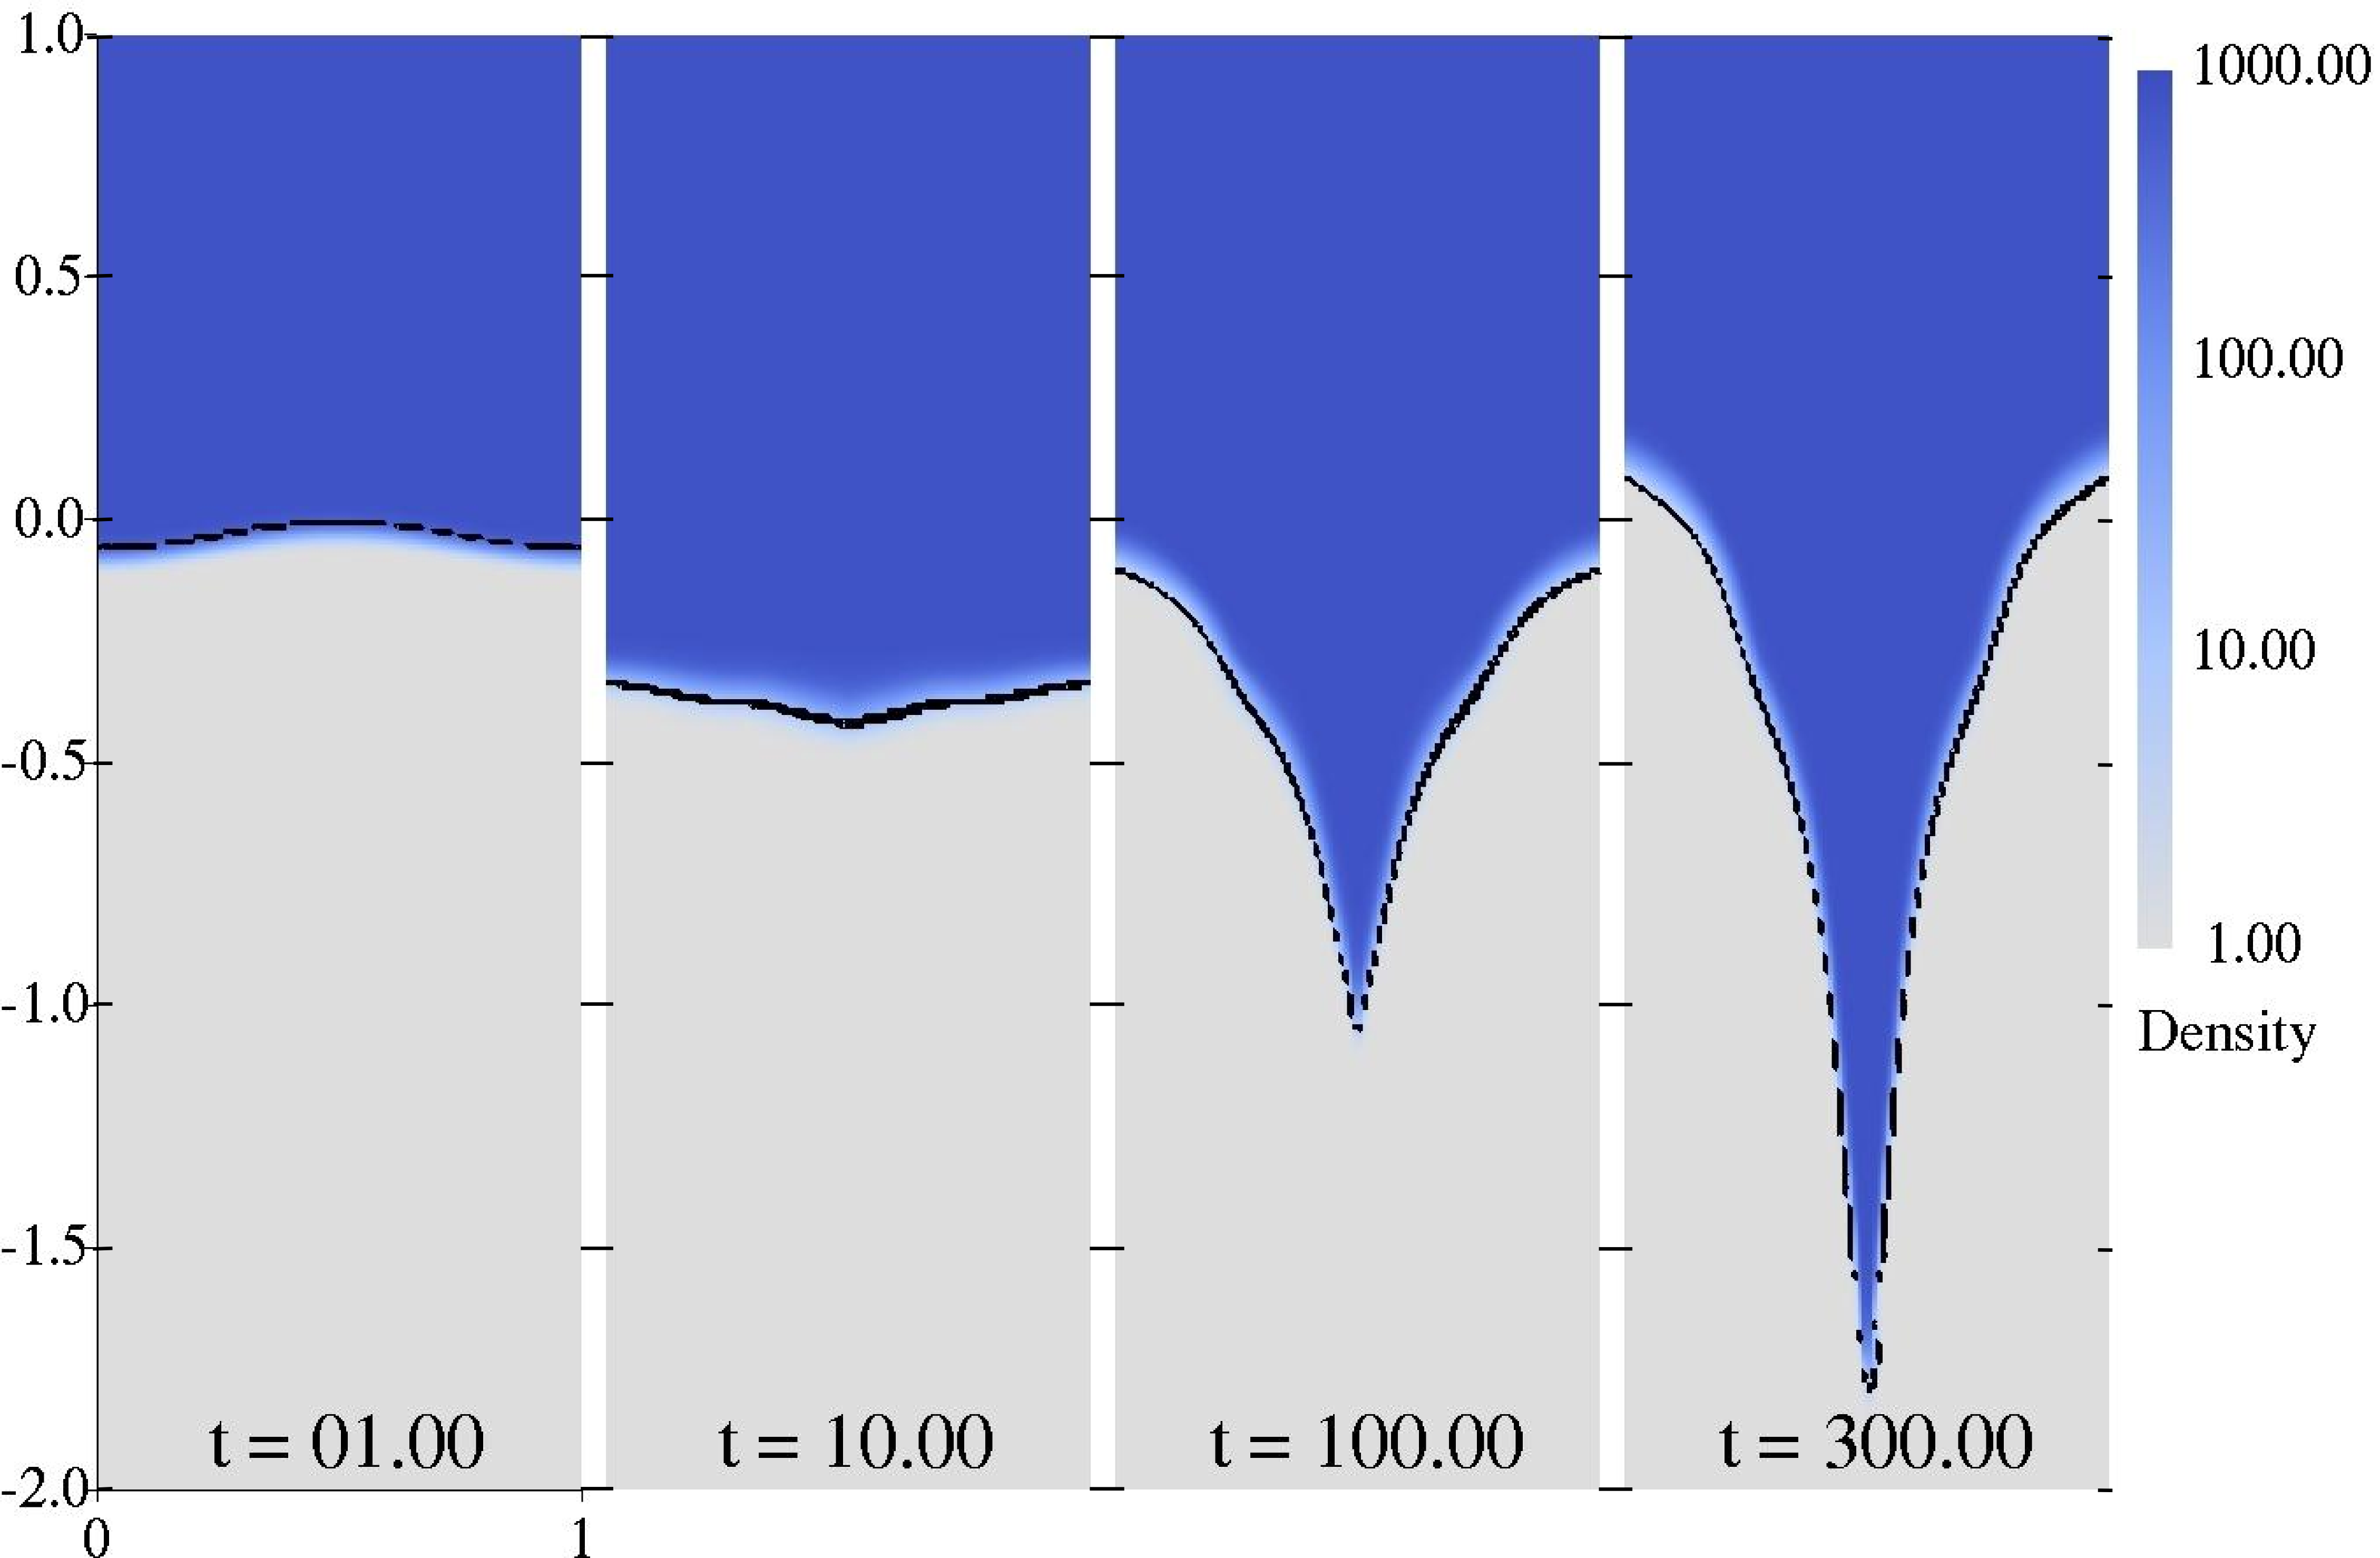
\includegraphics[width=0.9\textwidth]{./figs/lung_figs/snapshots_density_t1}
  \caption[The evolution of the acoustically perturbed interface]
  {Contour plots of density field illustrate the shape and location of
    the interface throughout the evolution of the flow, at
    $t=1, 10, 100, 300$, for the $10$ MPa trapezoidal wave case. Areas
    of high density (i.e., water) are indicated in dark blue. Areas of
    low density (i.e., air) are indicated in light blue. Constant volume
    fraction of water $y_0 = 0.5$ contour lines are indicated in black.}
  \label{fig:interface_snapshots}
\end{figure}
% 
To illustrate the evolution of the interface, Figure
\ref{fig:interface_snapshots} provides contour plots of the density
during the compression-interface interaction $(t=1)$, shortly after
the wave leaves the interface $(t=10)$, and at late times
$(t=100, 300)$. Note that all times and lengths presented are
dimensionless such that $t = \text{Time}/(\ell/c_{air}$ and $x$,
$y$ are nondimensionalized by $\ell$. High-density regions (i.e.,
water) are indicated in dark blue. Low-density regions (i.e., air) are
indicated in light-blue. Contours of volume fraction of water
$\alpha=0.5$ are indicated in black on both plots. The interface
perturbation grows from an initially smooth sinusoid to a sharp point
at late times, long after all waves have left the domain.
% 
\begin{figure}[h] 
  \centering
  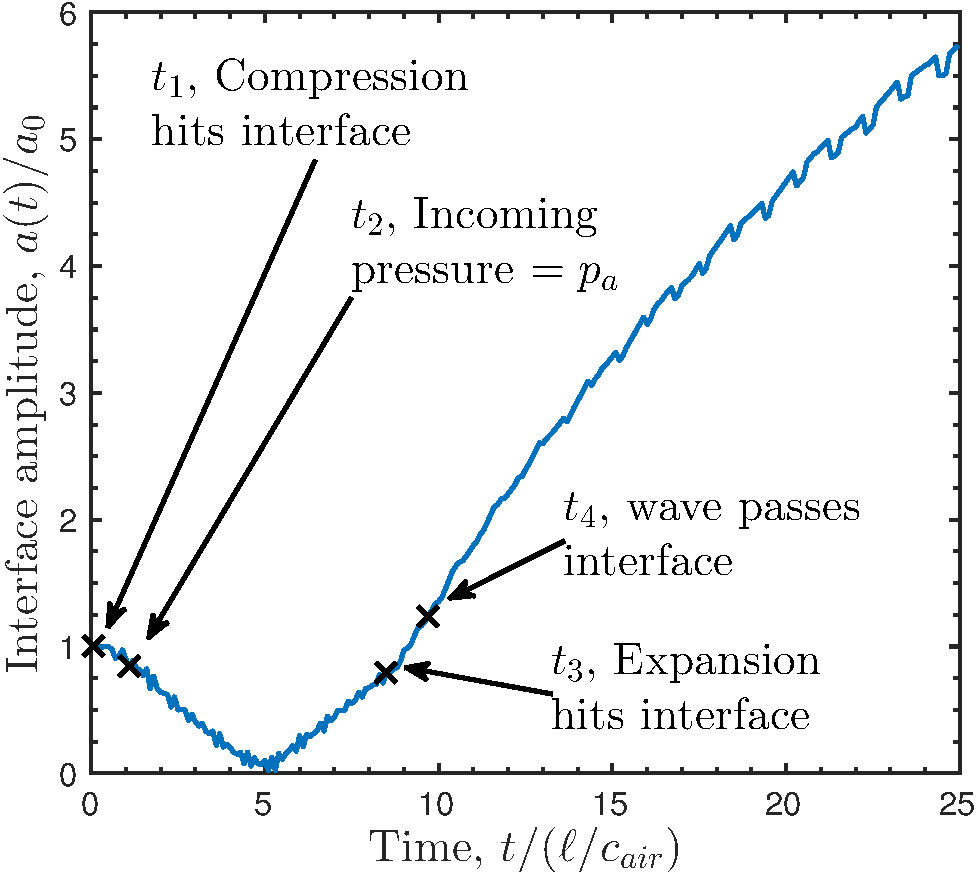
\includegraphics[width=0.48\textwidth]{./figs/lung_figs/trapz10_intf_schematic}
  ~
  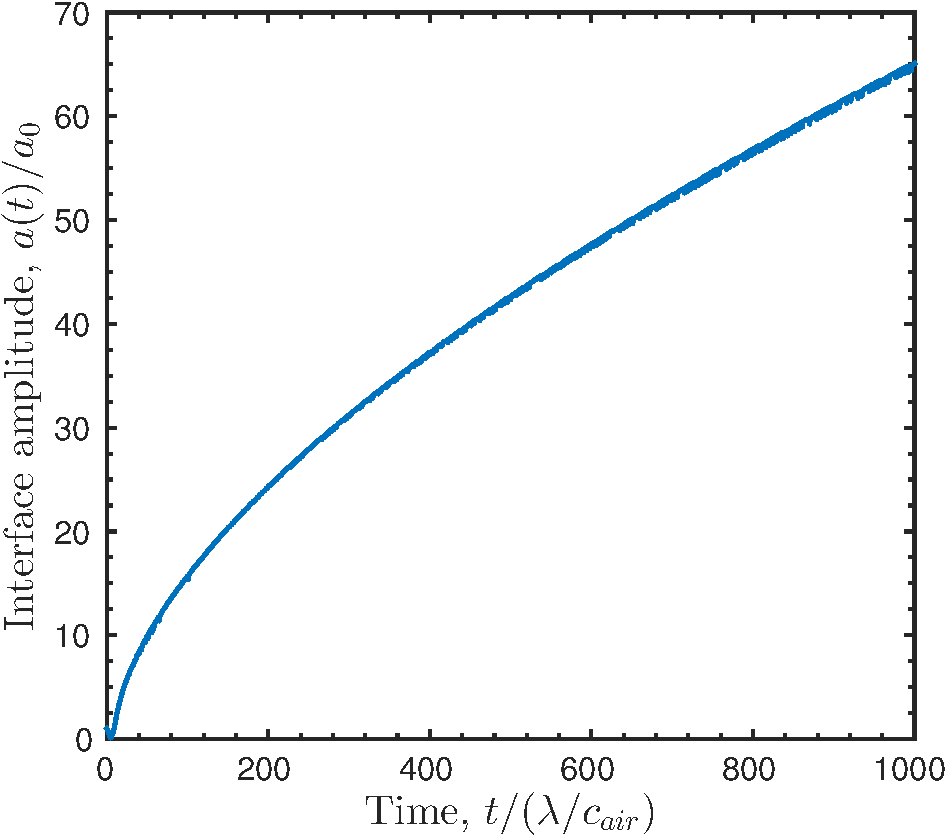
\includegraphics[width=0.48\textwidth]{./figs/lung_figs/interface_single-case_linear}%
  \caption[The interface perturbation amplitude history for 10 MPa]{The
    interface perturbation amplitude $a(t)$ for the $10$ MPa
    trapezoidal wave case for $t\leq25$ (Left) and $t\leq1000$ (Right). The times at which different
    stages of the incoming trapezoidal pressure wave encounter the
    interface are indicated as on the left plot as $t_{1-4}$.  }
  \label{fig:trapz10_interface}
\end{figure}\par
% 
To more closely exam the interface dynamics associated with the
wave-interface interaction, Figure \ref{fig:trapz10_interface} shows
the interface perturbation amplitude nondimensionalized by its initial
value $a(t)/a_0$ for $t\leq25$ and $t\leq1000$. We have labeled the times at which
different portions of the incoming wave encounter the interface as
$t_{1-4}$, denoted with black $\bs{\times}$s along the curves in these
figures and those hereafter. From $t_1=0^+$ to $t_2\approx1.1$ the
compression wave encounters the interface. At $t_2$, the incoming
pressure reaches its maximum amplitude, $p_a=10$ MPa, and remains
constant until $t_3\approx8.5$. During this period, the interface
amplitude continues to decrease until $t\approx 5.0$, at which point
the perturbation undergoes a phase inversion and begins to grow. This
phase inversion is similar to that observed for the heavy-light
interface Richtmyer-Meshkov problem. At $t_3$ the pressure expansion
hits the interface and the perturbation amplitude continues to
grow. At $t_4\approx9.7$ the acoustic wave has finished traversing the
interface, and the interface pressure is nominally atmospheric. In the
absence of viscosity or other loss mechanisms, the perturbation
amplitude $a(t)$ continues to increase indefinitely. After all waves
have left the domain, and the pressure is again uniformly atmospheric,
vorticity remains to drive the deformation of the interface.
% 
%%%%%%%%%%%%%%%%%%%%%%%%%%%%%%%%%%%%%%%%%%%%%%%%%%%%%%%%%%%%%%%%%% 
%%%%%%%%%%%%%%%%%%%%%%%%%%%%%%%%%%%%%%%%%%%%%%%%%%%%%%%%%%%%%%%%%% 
%%%%%%%%%%%%%%%%%%%%%%%%%%%%%%%%%%%%%%%%%%%%%%%%%%%%%%%%%%%%%%%%%% 
%%%%%%%%%%%%%%%%%%%%%%%%%%%%%%%%%%%%%%%%%%%%%%%%%%%%%%%%%%%%%%%%%% 
% 
\subsection{Vorticity and circulation dynamics}
\begin{figure}[h] 
  \centering
  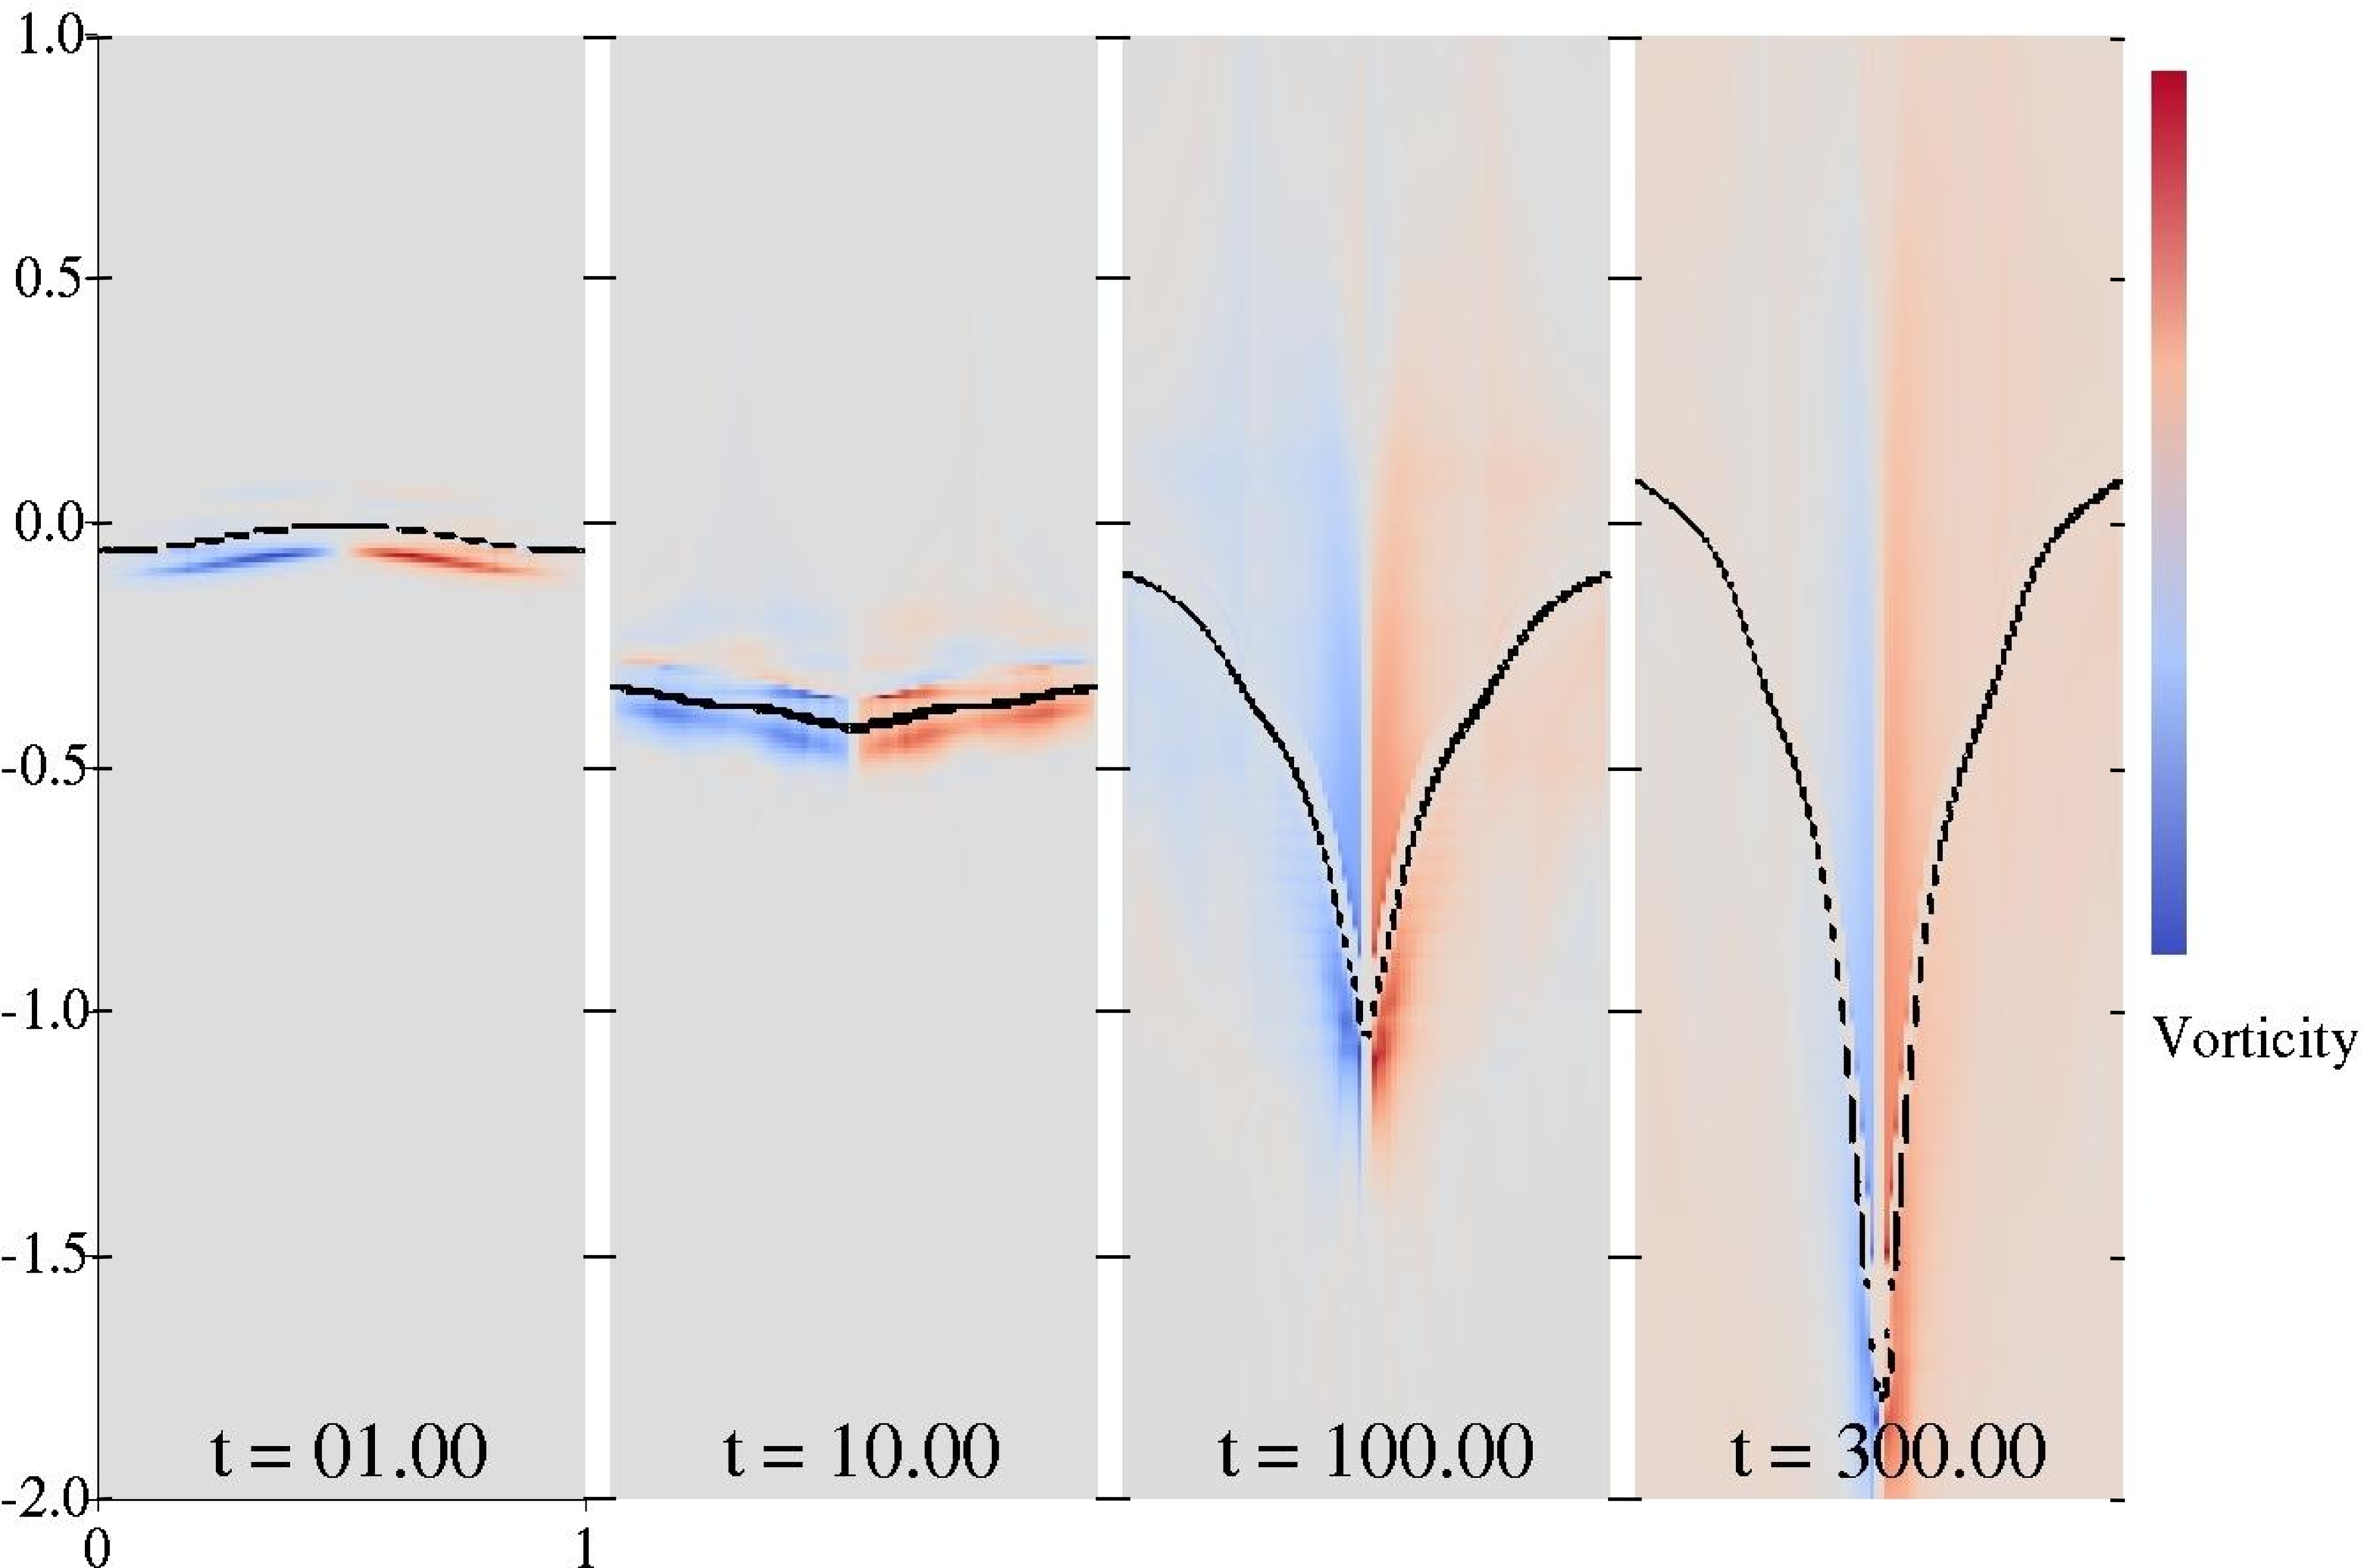
\includegraphics[width=0.9\textwidth]{./figs/lung_figs/snapshots_vorticity_t1}
  \caption[The evolution of the vorticity] {Contour plots of vorticity
    field throughout the evolution of flow, at
    $t=1, 10, 100, 300$, for the $10$ MPa trapezoidal wave case. Areas
    of positive vorticity are indicated in red. Areas of negative
    vorticity are indicated in blue. Constant volume fraction of 
    water $\alpha=0.5$ contour lines are indicated in black.}
  \label{fig:vorticity_snapshots}
\end{figure}
% 
To explain the continued growth of the interface at late times, we
look to the vorticity. Figure \ref{fig:vorticity_snapshots} shows
contour plots of the vorticity field at $t=1, 10, 100, 300$, for the
$10$ MPa trapezoidal wave case. Areas of positive (counter-clockwise)
vorticity are indicated in red. Areas of negative (clockwise)
vorticity are indicated in blue. As the purpose of this plot is to
visualize the location of vorticity, the color scale changes at each
time step and is not indicated on this plot. The position of the
interface is indicated by black contour lines of constant volume
fraction of water $\alpha=0.5$. At $t=1$, near the end of the
compression-interface interaction, the bulk of the vorticity is in
air-dominated fluid. As the perturbation grows, vorticity bleeds
across the interface. Vorticity remains concentrated around the middle
of the interface and in its wake.

To better understand the vorticity dynamics we consider the vorticity
generation equation for a 2D, inviscid fluid system,
\begin{align} \label{eq:vorticity_euler}
  \frac{\partial \boldsymbol{\omega}}{\partial t}+\left(\boldsymbol{u}\cdot\nabla\right)\boldsymbol{\omega} =% 
  - \boldsymbol{\omega}\left(\nabla\cdot\boldsymbol{u}\right) + \frac{\nabla\rho\times\nabla p}{\rho^2}.%
\end{align}

Each term in equation \eqref{eq:vorticity_euler} represents a
different physical mechanism by which the vorticity
$\boldsymbol{\omega}$ is changing. Terms on the left-hand side
represent changes in the existing vorticity field and terms on the
right represent vorticity sources and sinks. On the left, the first
term represents the total change of vorticity at a location in the
flow field with respect to time and the second term represents the
advection of vorticity. On the right, the first term describes changes
in vorticity due to compressibility, and the second term is the
baroclinic term which describes vorticity generated by the
misalignment of the pressure and density gradients. We
seek to understand the relative importance of these mechanisms on the
dynamics of the acoustically accelerated interface.
% 
%%%%%%%%%%%%%%%%%%%%%%%%%%%%%%%%%%%%%%%%%%%%%%%%%%%%%%%%%%%%%%%%%% 
%%%%%%%%%%%%%%%%%%%%%%%%%%%%%%%%%%%%%%%%%%%%%%%%%%%%%%%%%%%%%%%%%% 
%%%%%%%%%%%%%%%%%%%%%%%%%%%%%%%%%%%%%%%%%%%%%%%%%%%%%%%%%%%%%%%%%% 
%%%%%%%%%%%%%%%%%%%%%%%%%%%%%%%%%%%%%%%%%%%%%%%%%%%%%%%%%%%%%%%%%% 
% 
\subsubsection{Order of magnitude analysis of vorticity generation mechanisms}
\label{subsubsec:oom_analysis}
To quantifiably compare the various mechanisms by which vorticity
changes within the flow we perform an order of magnitude analysis on
each term of the vorticity generation equation
\eqref{eq:vorticity_euler}.

To determine the appropriate time and location for the analysis, we
recognize that the flow is initially free of vorticity and any
vorticity generated must be a result of acoustic energy being
converted to kinetic energy in the flow. The only mechanism for
this to occur in an inviscid fluid without pre-existing vorticity is
baroclinicity. Thus we require misaligned density and pressure
gradients. The greatest density gradients in the flow occur across the
interface. The strongest pressure gradients occur in the acoustic
wave. Hence we choose to perform our analysis at the water-air
interface during the period which is interacting with the incoming
wave.

For simplicity, we consider the period in which the compression
interacts with the interface. This interaction occurs
quickly, over approximately $\Delta t_a\approx5\ell/c_{w}$. As such
we treat the interface as static and undeformed during this
interaction. Based on the results presented in Figure
\ref{fig:trapz10_interface}, the average perturbation amplitude during
this period is $<a(t_{1-2})>\approx0.96\ a_0$, suggesting that this
assumption is reasonable for order of magnitude analysis.

To evaluate the order of magnitude of the individual terms of the
vorticity generation equation \eqref{eq:vorticity_euler}, we treat
gradient, curl, and divergence of any arbitrary quantity $f$ such that
$\abs{\nabla} f= \orderof{\left|\Delta f\right|/\Delta L}$,
$\nabla\cdot f=\orderof{\left|\Delta f\right|/\Delta L}$, and
$\nabla\times f=\orderof{\left|\Delta f\right|/\Delta L}$. Here
$\Delta f$ is a change in $f$ over a characteristic length scale
$\Delta L$. As the only motion in the flow is generated by the
acoustic wave, we consider acoustic pressure, velocity, and density
perturbations such that $\Delta p=\Delta p_a$,
$\Delta \boldsymbol{u}=\Delta \boldsymbol{u}_a$, and
$\Delta \rho=\Delta \rho_a$. The subscript $_a$ denotes acoustic
quantities. We use acoustic relations to relate these quantities
\citep{Anderson1990},
\begin{align}%
  \label{eq:acoustic_relations}%
  \Delta p_a=\pm\Delta u_a \rho c=c^2\Delta \rho_a.%
\end{align}

To assess the baroclinic contribution to vorticity, we write the cross
product of the density and pressure gradients as
$\abs{\nabla \rho} \abs{\nabla p} \sin{\left(\theta\right)}$. Here
$\theta$ is the angle between the acoustic pressure gradient, treated
as being in the $\plus y$-direction, and the direction of the density
gradient which we treat as the outward normal direction to the
interface. For $a_0/\ell<<1$, we can approximate
$\sin{\left(\theta\right)}\approx\theta$ at the interface. The density
gradient due to the water-air interface is far greater than that due
to the acoustic wave. As such we use the change in density across the
interface $\Delta \rho_I$ and associated length scale $\Delta L_I$ to
write the density gradient. The pressure change is a result of the
acoustic wave, and as such we use the acoustic pressure change
$\Delta p_a$ and associated length scale $\Delta L_a$ to express the
pressure gradient. And thus we write the order of magnitude of the
baroclinic vorticity generation term at the interface,
\begin{align}
  \label{eq:baroclinic_vorticity}%
  \norm{\frac{\nabla\rho\times\nabla p}{\rho^2}} =%
  \orderof{\frac{\abs{\Delta \rho_I}}{\abs{\Delta L_I}}\frac{\abs{\Delta p_a}}{\abs{\Delta L_a}}\frac{1}{\abs{\rho}^2}\abs{\theta}}.%
\end{align}

In the evaluation of the compressible and advective terms we consider
two possible evaluations of the vorticity $\omega$ as either the curl
of the acoustic velocity field
$\boldsymbol{\omega}=\nabla\times\boldsymbol{u}$ or the integral of
the baroclinic vorticity generation term from
\eqref{eq:baroclinic_vorticity}, treated as constant, over the
characteristic time of the pressure rise
$\Delta t_a\approx\Delta L_a/c_w$. Evaluating the vorticity using both
of these expressions and the values presented later in this section
reveals that the baroclinic expression of the vorticity is dominant
for the regimes of interest to this study and is thus what we will use
this treatment in our further analysis. Hence the approximate order of magnitude of the compressible and
advective vorticity generation is written as
\begin{align}
  \label{eq:compressible_advective_vorticity}%
  \norm{-\boldsymbol{\omega}\left(\nabla\cdot\boldsymbol{u}\right)}\sim \norm{\left(\boldsymbol{u}\cdot\nabla\right)\boldsymbol{\omega}} = %
  \orderof{%
  \frac{\abs{\Delta u_a}}{\abs{\Delta L_a}} \frac{\abs{\Delta \rho_I}}{\abs{\Delta L_I}}%
  \frac{\abs{\Delta p_a}}{\abs{\Delta L_a}} \frac{1}{\abs{\rho}^2}\abs{\theta}\frac{\abs{c}}{\abs{\Delta L_a}}%
  }.%
\end{align}

Now, to compare the relative importance of the baroclinic and
compressible (or advective) contributions to vorticity we will look at
the ratio of the two vorticity generation approximations. We divide
equation \eqref{eq:baroclinic_vorticity} by equation
\eqref{eq:compressible_advective_vorticity} using
\eqref{eq:acoustic_relations} to express acoustic quantities in terms
of the acoustic perturbation quantities $\Delta \rho_a,\,\Delta u_a$ and simplify,
\begin{align} \label{eq:vorticity_comparison}
  \frac{\norm{\frac{\nabla\rho\times\nabla
  p}{\rho^2}}}{\norm{-\boldsymbol{\omega}\left(\nabla\cdot\boldsymbol{u}\right)}}
  \sim
  \frac{\norm{\frac{\nabla\rho\times\nabla
  p}{\rho^2}}}{\norm{\left(\boldsymbol{u}\cdot\nabla\right)\boldsymbol{\omega}}}
  = \orderof{\frac{\abs{c}}{\abs{\Delta u_a}}} = \orderof{\frac{\abs{\rho}}{\abs{\Delta \rho_a}}}%
\end{align}

To evaluate the above expressions for comparison with our
computational results, we consider our base trapezoidal wave case
where $p_a = \Delta p_a = 10$ MPa. The length scale associated with
the acoustic wave is the initial length of the pressure rise
$\Delta L_a=5\ell$. The initial interface length scale
$\Delta L_I$, defined as the thickness of the thickness of the mixed
layer from $\alpha=0.05$ to $0.95$ volume fraction of water is estimated
as $\Delta L_I \approx 0.05\ell$. We approximate the order of theta
based on its average value along a half-wavelength of the interface
for $a_0=0.03\ell$ such that
$<\abs{\theta}>\approx0.12$. Evaluating expression
\eqref{eq:vorticity_comparison} we to find that
$\abs{c}/\abs{\Delta u_a}$=247 and thus expect that the relative
contribution of baroclinic to compressible/advective vorticity
generation is approximately of order $\orderof{10^2}$ at
$t=\Delta t_a=1.05$.

To compare our computational results to the analysis we consider the
integral of the vorticity and vorticity generation terms over the
right-half domain,
\begin{align}
  \Gamma = \int_{A_{RH}} \omega \,dA_{RH},
\end{align}
where
$\int_{A_{RH}} dA_{RH} =
\int_{-\infty}^{+\infty}\int_{\ell/2}^{\ell} \,dy\, dx$. Note
that the right-half domain is considered because the total circulation
over the whole domain is $0$ due to symmetry. Circulation is chosen as
the quantity of comparison as it is a global quantity, which better
captures the overall vorticity dynamics than the vorticity at any
single point. As a single quantity rather than a field, it is also
simpler to compare the computational and analytical results. The
relative order of magnitude relationships obtained in
\eqref{eq:vorticity_comparison} are spatially independent and expected
to hold when integrated over the right-half domain. Accordingly we
evaluate the vorticity generation terms from our computational results
integrated over the right-half domain. At $t=1.0$ we find that %
$$ \int_{A_{RH}} \left[\frac{\nabla\rho\times\nabla p}{\rho^2}\right] / \left[\left(\boldsymbol{u}\cdot\nabla\right)\boldsymbol{\omega}\right]\,\,dA_{RH}\approx 285=\orderof{10^2}$$
and
$$ \int_{A_{RH}} \left[\frac{\nabla\rho\times\nabla p}{\rho^2}\right] / \left[-\boldsymbol{\omega}\left(\nabla\cdot\boldsymbol{u}\right)\right]\,\,dA_{RH} \approx 145=\orderof{10^2}.$$%
% %
% \begin{comment} %This shows actual values instead of relative ones
% $ \int_{A_{RH}} \left(\frac{\nabla\rho\times\nabla p}{\rho^2}\right)
% \,\,dA_{RH}= 7.7\,\text{e}{-3}$, %
% $ \int_{A_{RH}} \left(\boldsymbol{u}\cdot\nabla\right)\boldsymbol{\omega}\,\,dA_{RH}
% = -5.3\text{e}{-5}$, and %
% $ \int_{A_{RH}}
% -\boldsymbol{\omega}\left(\nabla\cdot\boldsymbol{u}\right)\,\,dA_{RH} =
% 2.7\text{e}{-5}$.%
% \end{comment}
%
Hence the computational results and analysis are in agreement and suggest
that the vorticity is nearly entirely baroclinic.
% 
%%%%%%%%%%%%%%%%%%%%%%%%%%%%%%%%%%%%%%%%%%%%%%%%%%%%%%%%%%%%%%%%%% 
%%%%%%%%%%%%%%%%%%%%%%%%%%%%%%%%%%%%%%%%%%%%%%%%%%%%%%%%%%%%%%%%%% 
%%%%%%%%%%%%%%%%%%%%%%%%%%%%%%%%%%%%%%%%%%%%%%%%%%%%%%%%%%%%%%%%%% 
%%%%%%%%%%%%%%%%%%%%%%%%%%%%%%%%%%%%%%%%%%%%%%%%%%%%%%%%%%%%%%%%%% 
% 
\subsubsection{Circulation deposition}
Having established that the circulation is a primarily result of
baroclinic vorticity, we now look to understand the circulation
deposition associated with the wave-interface interaction period.

\begin{figure}[h] 
  \centering
  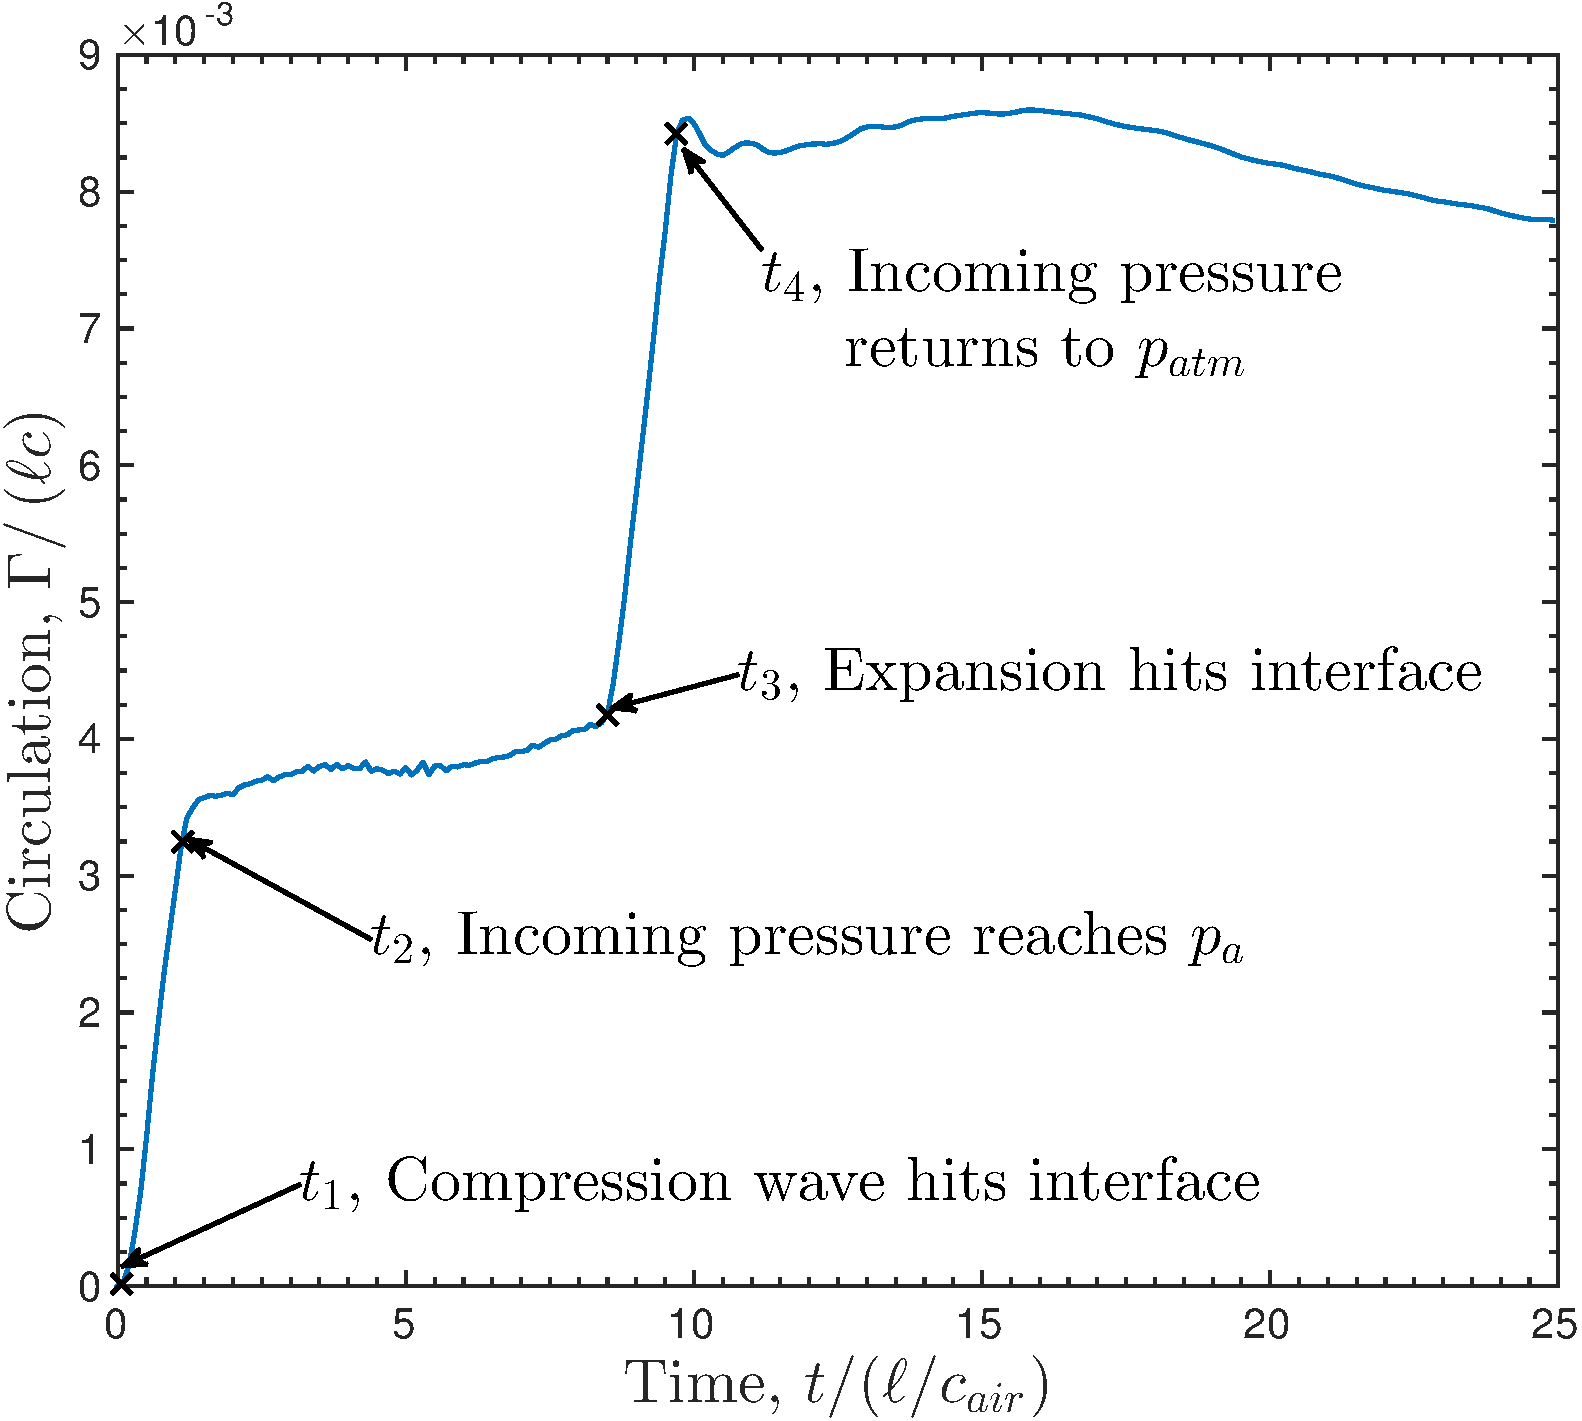
\includegraphics[height=0.3\textheight]{./figs/lung_figs/trapz10_circ_schematic}
  \caption[Circulation deposition by the 10 MPa trapezoidal wave] {The
    circulation history for the right-half domain is shown for the 10
    MPa trapezoidal wave case for $t\leq25$. The times at which
    different stages of the incoming trapezoidal pressure wave
    encounter the interface are indicated as $t_{1-4}$.}
  \label{fig:trapz10_circ_schematic}
\end{figure}

Figure \ref{fig:trapz10_circ_schematic}, shows right-half domain
circulation history for the $10$ MPa wave case for $t\leq25$, during
and shortly after the wave-interface interaction. Black $\bs{\times}$s
along the curves indicate $t_{1-4}$, as described in
section \ref{subsec:Qualitative}.

From $t_1=0^+$ to $t_2$ the compression wave encounters the interface
and $\Gamma$ increases. From $t_2\approx1.1$ to $t_3\approx8.5$ the
pressure gradient at the interface is small and $\Gamma$ changes
little. From Figure \ref{fig:trapz10_interface}, the perturbation
undergoes a phase inversion at $t\approx 5.0$, and hence the density
gradient along the interface reverses direction around this point in
time. At $t_3\approx8.5$ the expansion wave first hits the
interface. The pressure and density gradients at the interface have
both reversed sign since the initial compression wave-interface
interaction and $\Gamma$ increases sharply again. At
$t_4\approx9.7$ the acoustic wave has finished traversing the
interface and ceases depositing vorticity around the interface.

\subsubsection{Circulation-driven, late-time growth of the interface}
\begin{figure}[h]
  \centering
  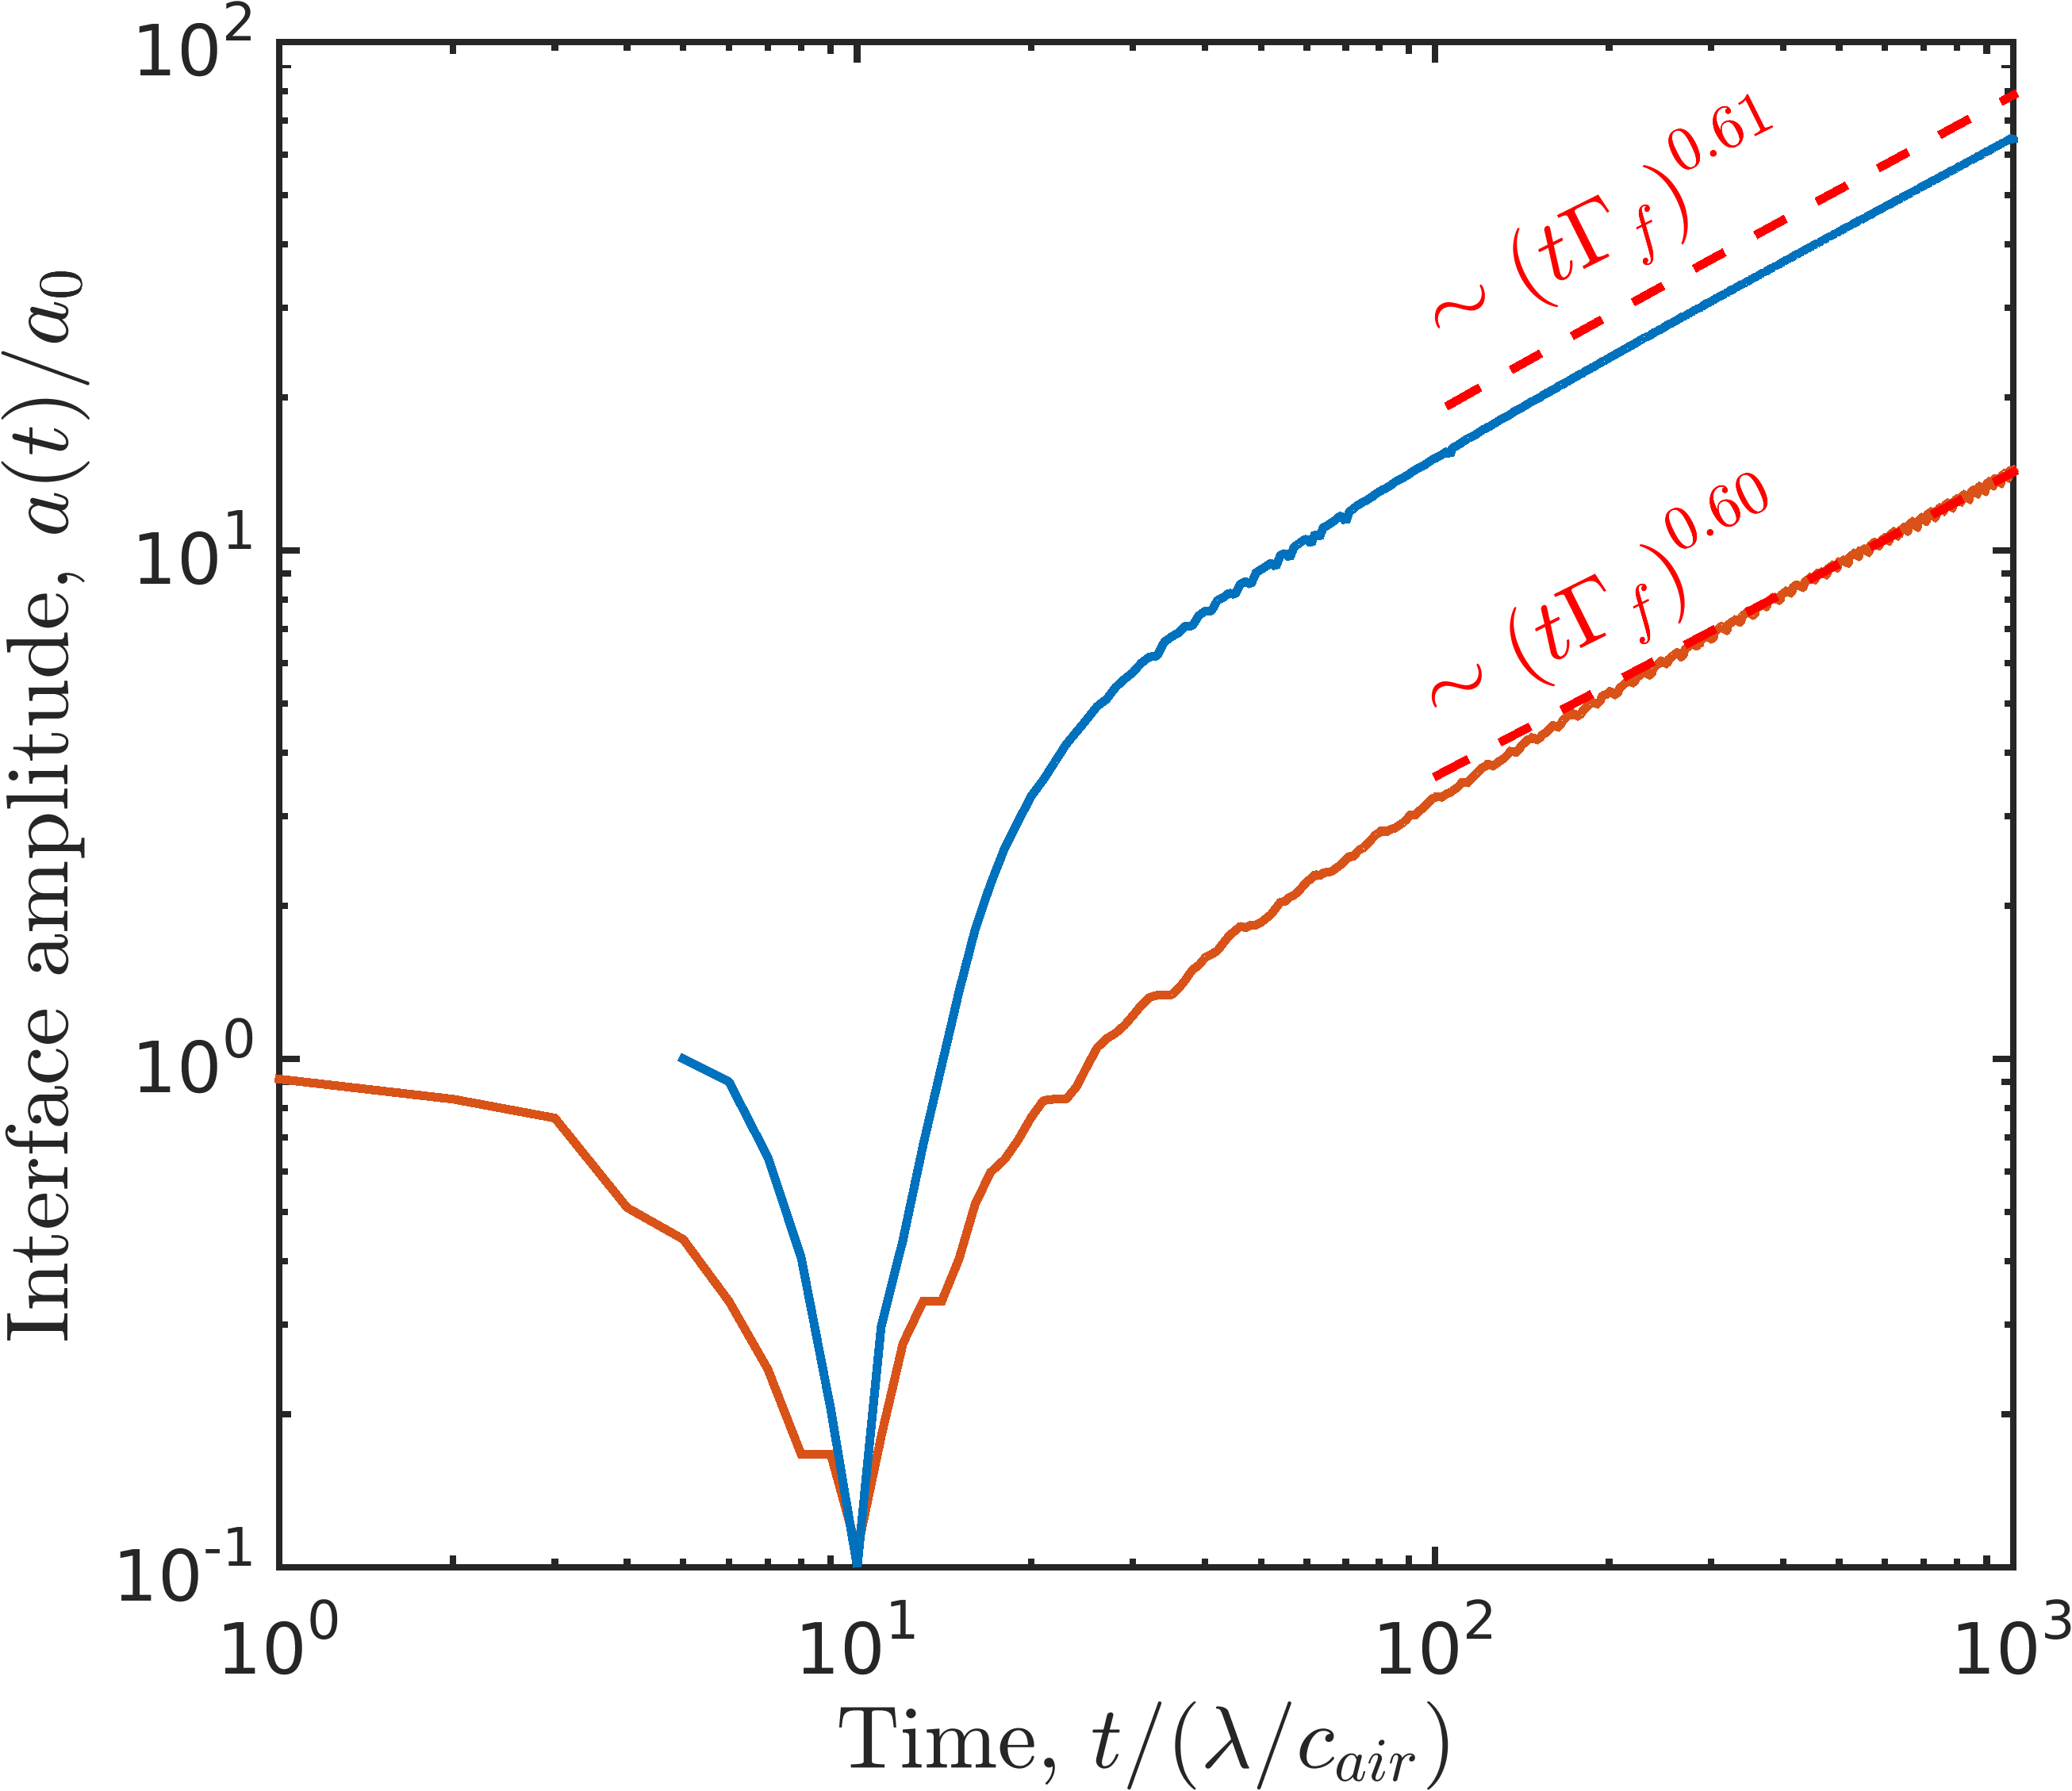
\includegraphics[width=0.48\textwidth]{./figs/lung_figs/interface_multi-amp_loglog_roe_t1000}
  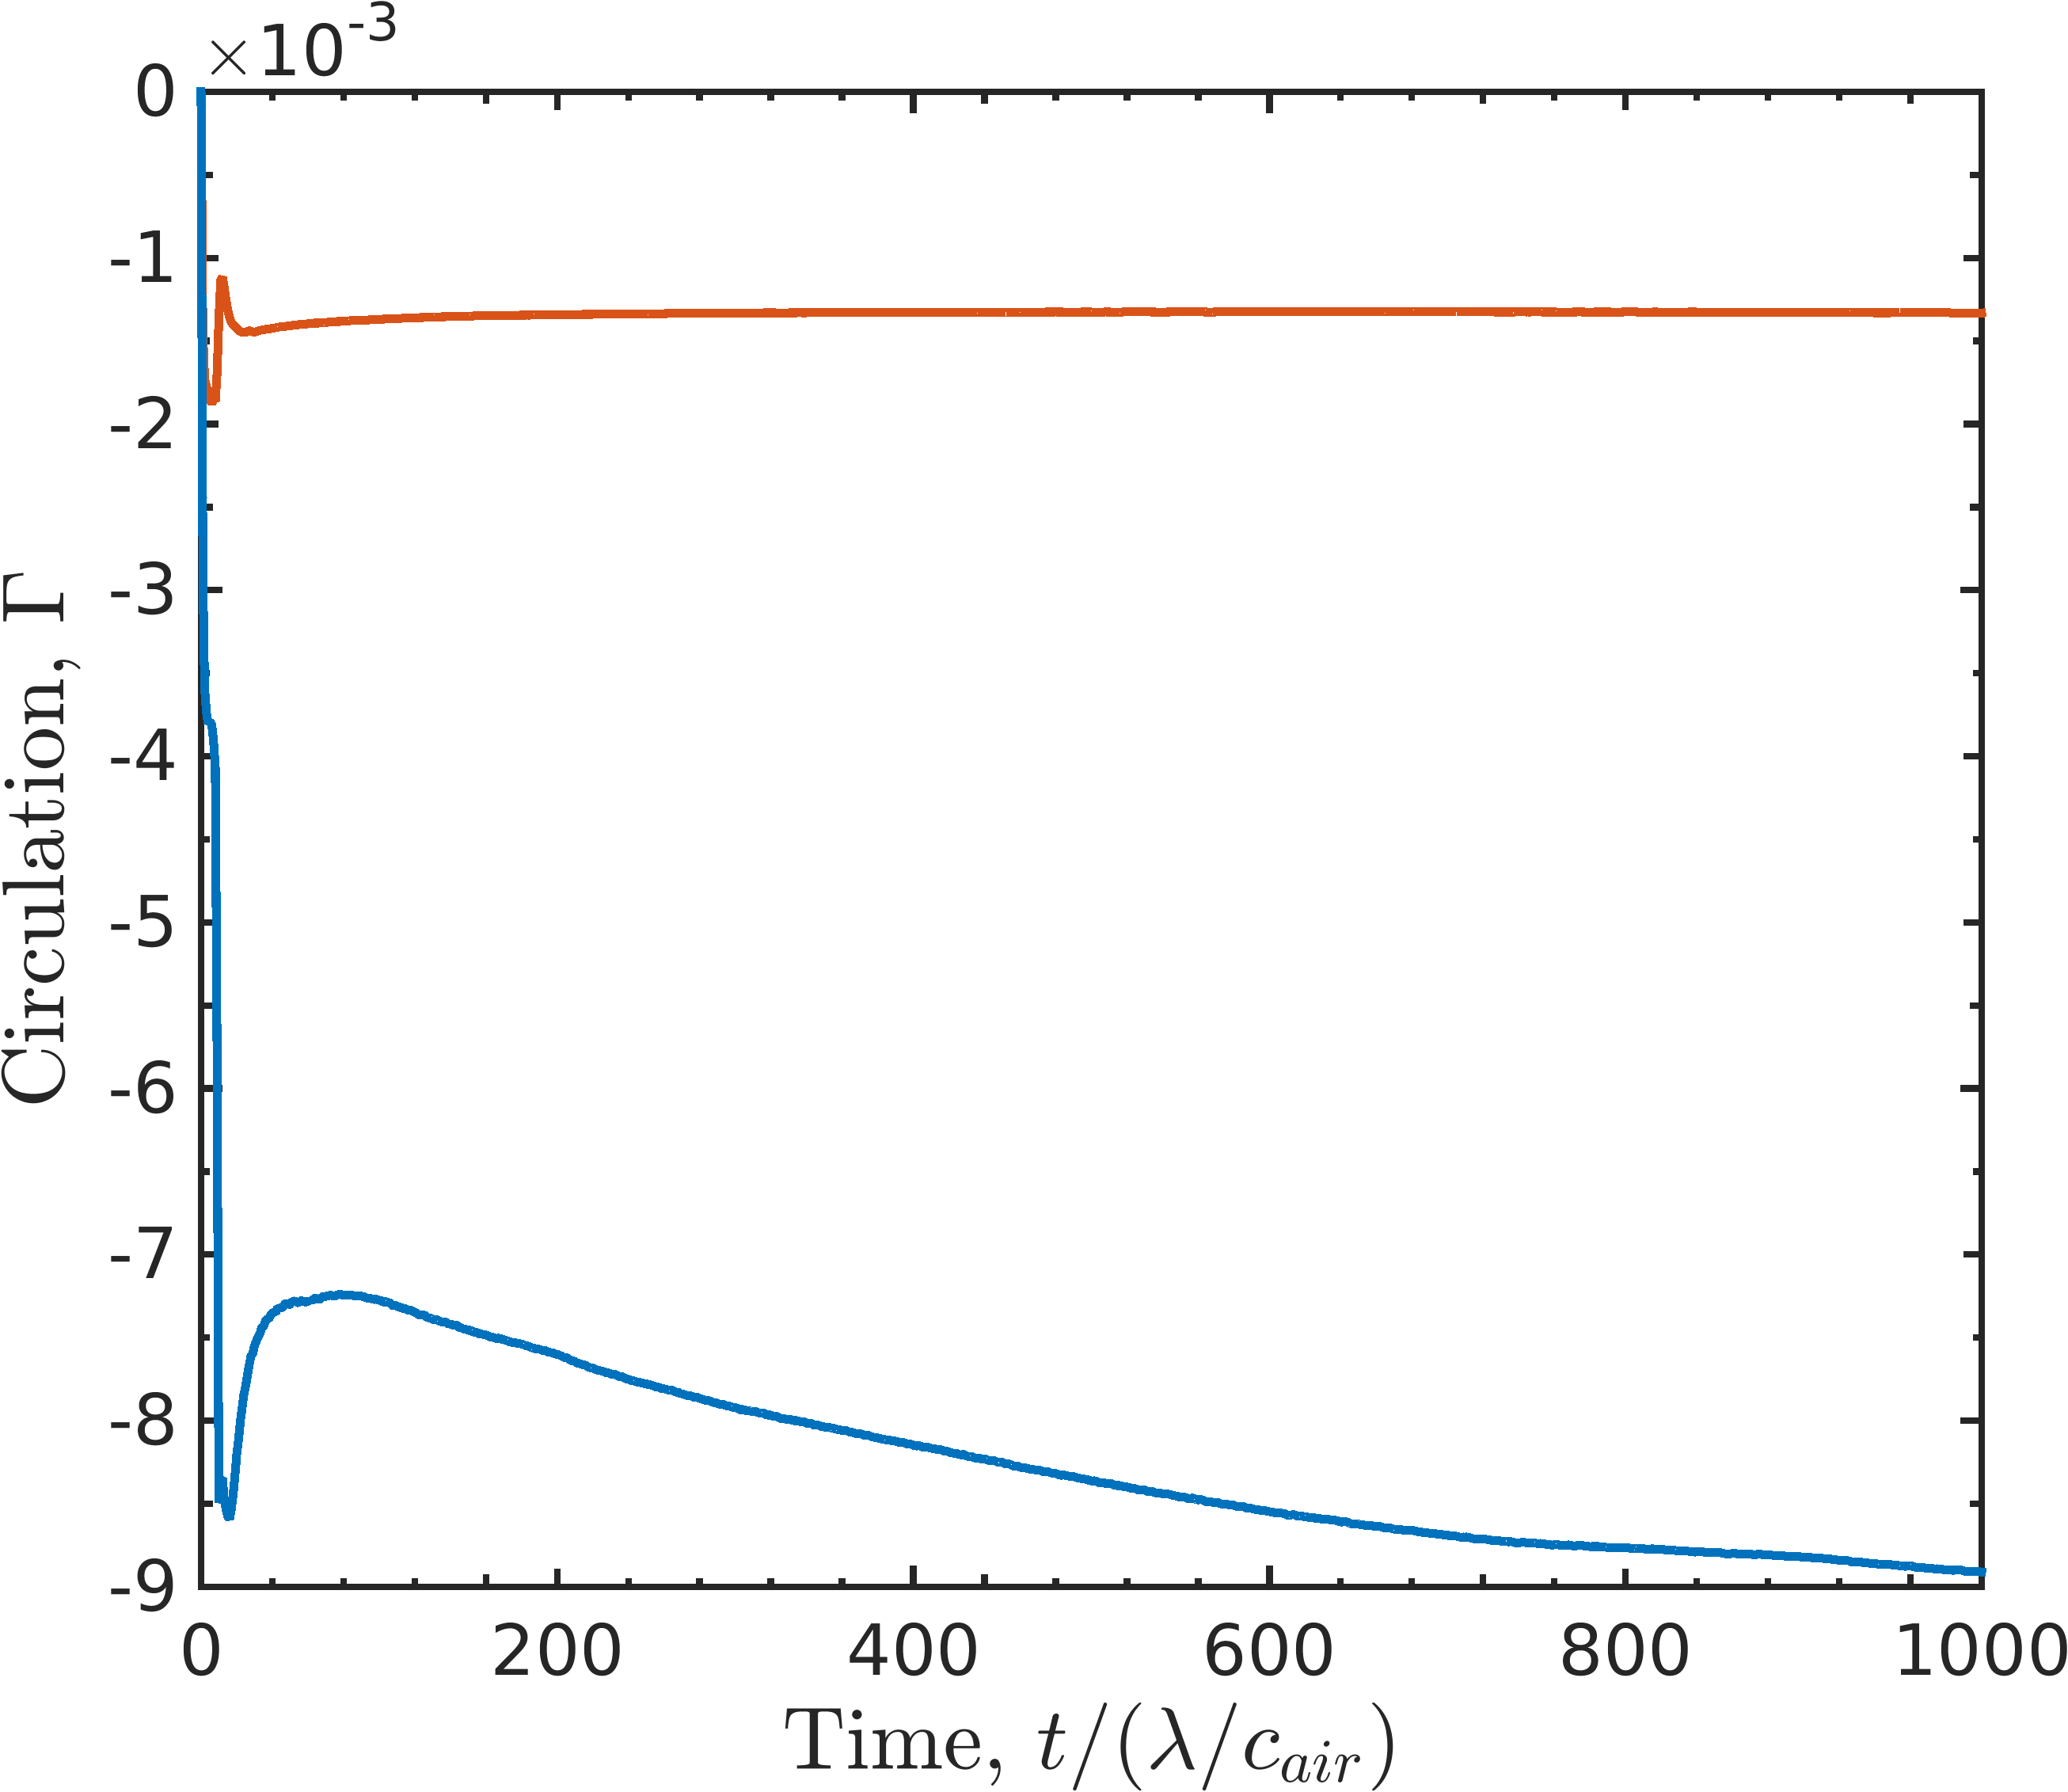
\includegraphics[width=0.48\textwidth]{./figs/lung_figs/circulation_multi-amp_roe_t1000}
  \caption[The interface and circulation dependence on wave amplitude
  at long time]{The interface amplitude (left) and circulation (right)
    histories corresponding to the $5$(orange), $10$(blue), and
    \hl{$15$ (?)} MPa trapezoidal waves are shown for $t\leq 1000$. To
    compare perturbation amplitudes $a(t)/a_0$ at late time,
    time has been offset for each case such that the phase reversal appears to occur
    simultaneously. Dashed red lines to demonstrate the best fit
    curves for power law growth.}
  \label{fig:trapz_circ_interface_loglog}
\end{figure}
% 
Figure \ref{fig:trapz_circ_interface_loglog} \hl{(update this figure
  w/ $15$ MPa case)} shows the interface amplitude and circulation
histories for $5$, $10$, and $15$ MPa trapezoidal wave cases for
$0 \leq t\leq 1000$. The perturbation amplitude history is plotted on
logarithmically-scaled axes such that the constant slope at late times
suggests power law growth. Using dimensional analysis it is simple
to show that for a purely-circulation-driven interface perturbation
% 
\begin{align} \label{eq:intf_circ_scaling}
  a(t) \sim \sqrt{\Gamma t}.
\end{align}
% 
For \hl{all cases considered}, the slope of the perturbation amplitude
is approximately $0.6$ long after the waves have left the
interface. This is slightly faster than the $t^{0.5}$ growth predicted by
dimensional analysis. 
% 
%%%%%%%%%%%%%%%%%%%%%%%%%%%%%%%%%%%%%%%%%%%%%%%%%%%%%%%%%%%%%%%%%% 
%%%%%%%%%%%%%%%%%%%%%%%%%%%%%%%%%%%%%%%%%%%%%%%%%%%%%%%%%%%%%%%%%% 
%%%%%%%%%%%%%%%%%%%%%%%%%%%%%%%%%%%%%%%%%%%%%%%%%%%%%%%%%%%%%%%%%% 
%%%%%%%%%%%%%%%%%%%%%%%%%%%%%%%%%%%%%%%%%%%%%%%%%%%%%%%%%%%%%%%%%% 
% 
To better understand the distribution of vorticity generation within
the gas-liquid mixture region of the interface we perform an order of
magnitude analysis to compare the baroclinic vorticity from equation
\eqref{eq:baroclinic_vorticity} in pure water vs air. As this can
already be evaluated in water from what we have provided up to this
point, we will focus on evaluation of the order of baroclinic
vorticity generation in air.

Throughout this analysis we will denote the properties of the incoming
wave and water with a subscript $-$, and the transmitted wave and air
with a subscript $+$. For water, we will use the values for
$\Delta \rho_I, \Delta L_I, \Delta \rho_a, \Delta L_a$ and $\theta$
previously defined in the section \ref{subsubsec:oom_analysis}, based
on our initial condition. Our treatment of the density gradient across
the interface will remain unchanged for evaluation in air such that
$\Delta \rho_I^-=\Delta \rho_I^+$ and $\Delta L_I^-=\Delta L_I^+$. To
evaluate the remaining terms in air we will borrow techniques from
linear acoustics. To find the pressure rise in the transmitted wave
$\Delta p_a^+$, we recognize that $a_0/\ell<<1$ and treat the
incoming wave as a plane wave impinging normally on a flat material
interface such that $\Delta p_a^+=\bs{T} \Delta p_a^-$, where $\bs{T}$
is the acoustic transmission coefficient,
$\bs{T}=2\rho^+ c^+/\left(\rho^+ c^+ + \rho^- c^- \right)$
\citep{Kinsler1982}. For our water-air interface
$\bs{T}\approx4.97\times10^{-4}$. Because of the strong impedance
mismatch between fluids, the acoustic wave is almost entirely
reflected, decreasing the pressure gradient in the air. Because of the
drop in sound speed across the interface, the transmitted wave is
compressed into a smaller physical area (i.e., the wavelength
decreases) relative to the incoming wave, such that
$\Delta L_a^+=\Delta L_a^- (c^+/c^-)$. This effect increases the
pressure gradient in the air. To evaluate $\theta^+$, we utilize
Snell's law which states that
$c^-\sin{\theta^-}=c^+\sin{\theta^+}$. Because $a_0/\ell<<1$ it is
also true that $\theta^-<<1$, thus we use the small angle
approximation of $\sin$ to find that
$\theta^+\approx\theta^-(c^+/c^-)$. This refraction effect decreases
the misalignment between the pressure and density gradients for the
transmitted wave relative to the incoming wave. Quantitatively it also
approximately cancels the increase in vorticity deposition that arises
as a result of the increased pressure gradient created by the decrease
in the length of the transmitted wave.

To get an idea of where within the mixed gas-liquid region at the
interface the vorticity will be generated, we consider equation
\eqref{eq:baroclinic_vorticity} in air and water and write the ratio
to find
\begin{align}%
  \label{eq:baroclinic_air_water}%
  % \left(\frac{\partial\omega}{\partial t}\right)_{\substack{\text{baroclinic}\\\text{air}}} / \left(\frac{\partial\omega}{\partial t}\right)_{\substack{\text{baroclinic}\\\text{water}}}%
  \frac{\norm{\frac{\nabla\rho\times\nabla p}{\rho^2}}_{air\quad}}{\norm{\frac{\nabla\rho\times\nabla p}{\rho^2}}_{water}}
  =&\orderof{\frac{\left[\frac{\abs{\Delta \rho_I^+}}{\abs{\Delta L_I^+}}\frac{\abs{\Delta p_a^+}}{\abs{\Delta L_a^+}}\frac{1}{\abs{\rho^+}^2}\abs{\theta^+}\right]}
     {\left[\frac{\abs{\Delta \rho_I^+}}{\abs{\Delta L_I^+}}\frac{\left(\abs{\Delta p_a^+}/\abs{\bs{T}}\right)}{\abs{\Delta L_a^+}\left(\abs{c^+}/\abs{c^-}\right)}\frac{1}{\abs{\rho^-}^2}\left(\abs{c^+}/\abs{c^-}\right)\abs{\theta^+}\right]}},\nonumber\\%
  =&\orderof{\abs{\bs{T}}\left(\frac{\abs{\rho^-}}{\abs{\rho^+}}\right)^2}.%
\end{align}
For our water-air interface, we evaluate equation
\eqref{eq:baroclinic_air_water} to find that the ratio of baroclinic
vorticity generation in air to that in water would be of order
$\orderof{10^2}$. While this analysis considers vorticity generation
in pure air and water, as opposed to the mixed fluid region that is
exactly relevant to this work, we make two observations based on this
result. First, this result analysis is for an extreme case in which
all of the vortical energy relevant to this problem, is able to be
concentrated in pure air and water, and thus this result acts as an
upper bound on the change in vorticity deposition we expect as the
wave move from water across the interface into air. Additionally, this
result suggests that for the mixed water-air region, where the
strongest density gradient exists, vorticity generation is likely to
occur in gas dominated fluid regions with a higher volume fraction of
air than water.
\begin{figure}[h]
  \centering
  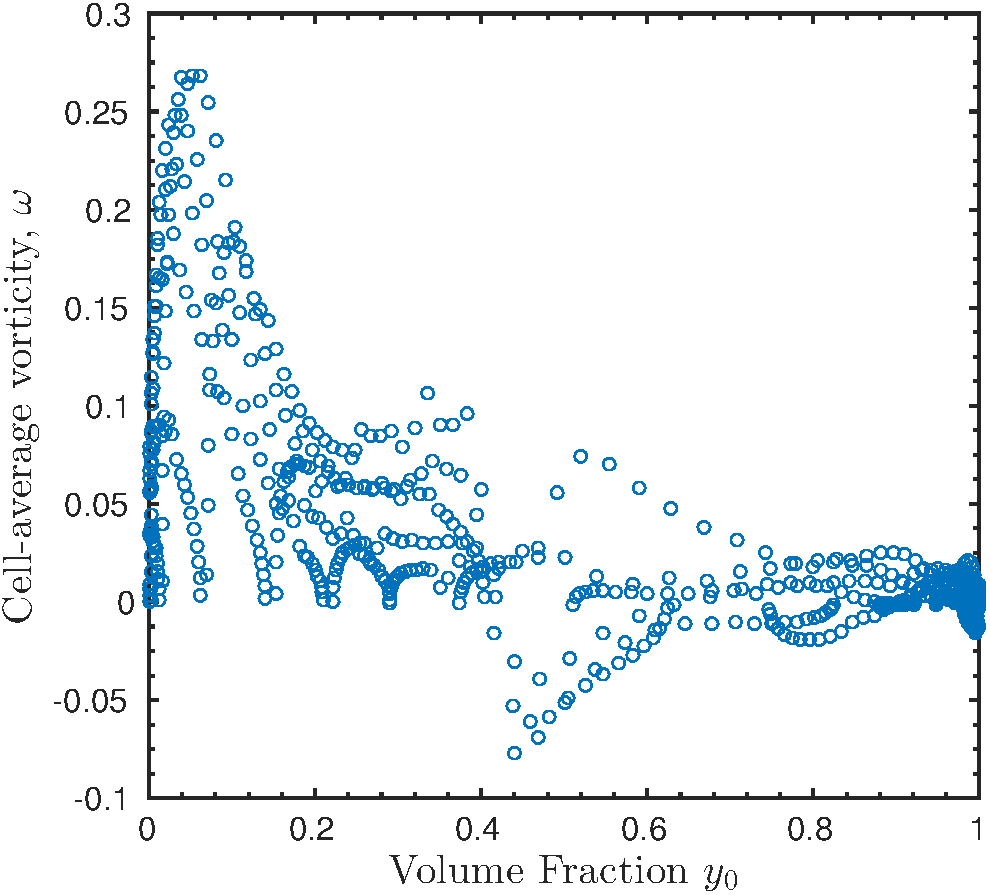
\includegraphics[width=.48\textwidth]{./figs/lung_figs/vorticity_vs_y0} \hfill
  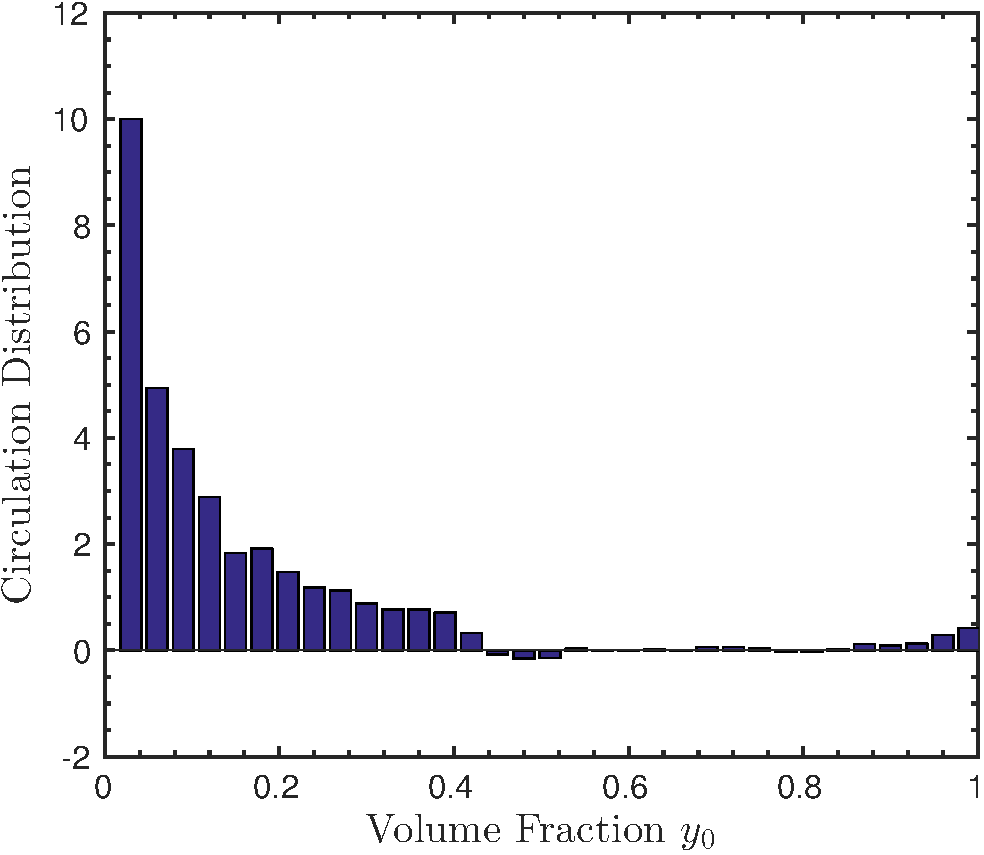
\includegraphics[width=.48\textwidth]{./figs/lung_figs/circ_y0_dist2}
  \caption{For cells with non-negligible vorticity, a scatter plot of the mean vorticity in each cell is plotted as a function of volume fraction water (Left).  }
  \label{fig:baroclinic_y0_distribution}  
\end{figure}

From the vorticity contours at $t=1.0$ shown in
\ref{fig:vorticity_snapshots}, the vorticity is clearly concentrated
in the region with volume fraction of water $\alpha<0.5$. To quantify
this, numerically integrating the vorticity over the right-half domain
we find that 97\% of the circulation occurs in this region. To further
illustrate the dependence of the vorticity deposition on the relative
gas-liquid composition of the fluid within the interface region,
Figure \ref{fig:baroclinic_y0_distribution} shows a scatter plot of
the vorticity values in each cell vs the mean volume fraction of water
in the cell $<\alpha>$ (Left). The average circulation per-cell is
seperated into bins based on the relevant volume fraction to obtain a
histogram and normalized to obtain the circulation distribution
circulation as a function of $\alpha$ (Right). The observed circulation
deposition in air-dominated fluid, $\alpha<0.5$, and is within the
predicted upper bound. This is qualitatively consistent with our
analysis.
% 
%%%%%%%%%%%%%%%%%%%%%%%%%%%%%%%%%%%%%%%%%%%%%%%%%%%%%%%%%%%%%%%%%% 
%%%%%%%%%%%%%%%%%%%%%%%%%%%%%%%%%%%%%%%%%%%%%%%%%%%%%%%%%%%%%%%%%% 
%%%%%%%%%%%%%%%%%%%%%%%%%%%%%%%%%%%%%%%%%%%%%%%%%%%%%%%%%%%%%%%%%% 
%%%%%%%%%%%%%%%%%%%%%%%%%%%%%%%%%%%%%%%%%%%%%%%%%%%%%%%%%%%%%%%%%% 
% 
\subsubsection{Dependence on the length of the wave}%
\begin{figure}[h]
  \centering
  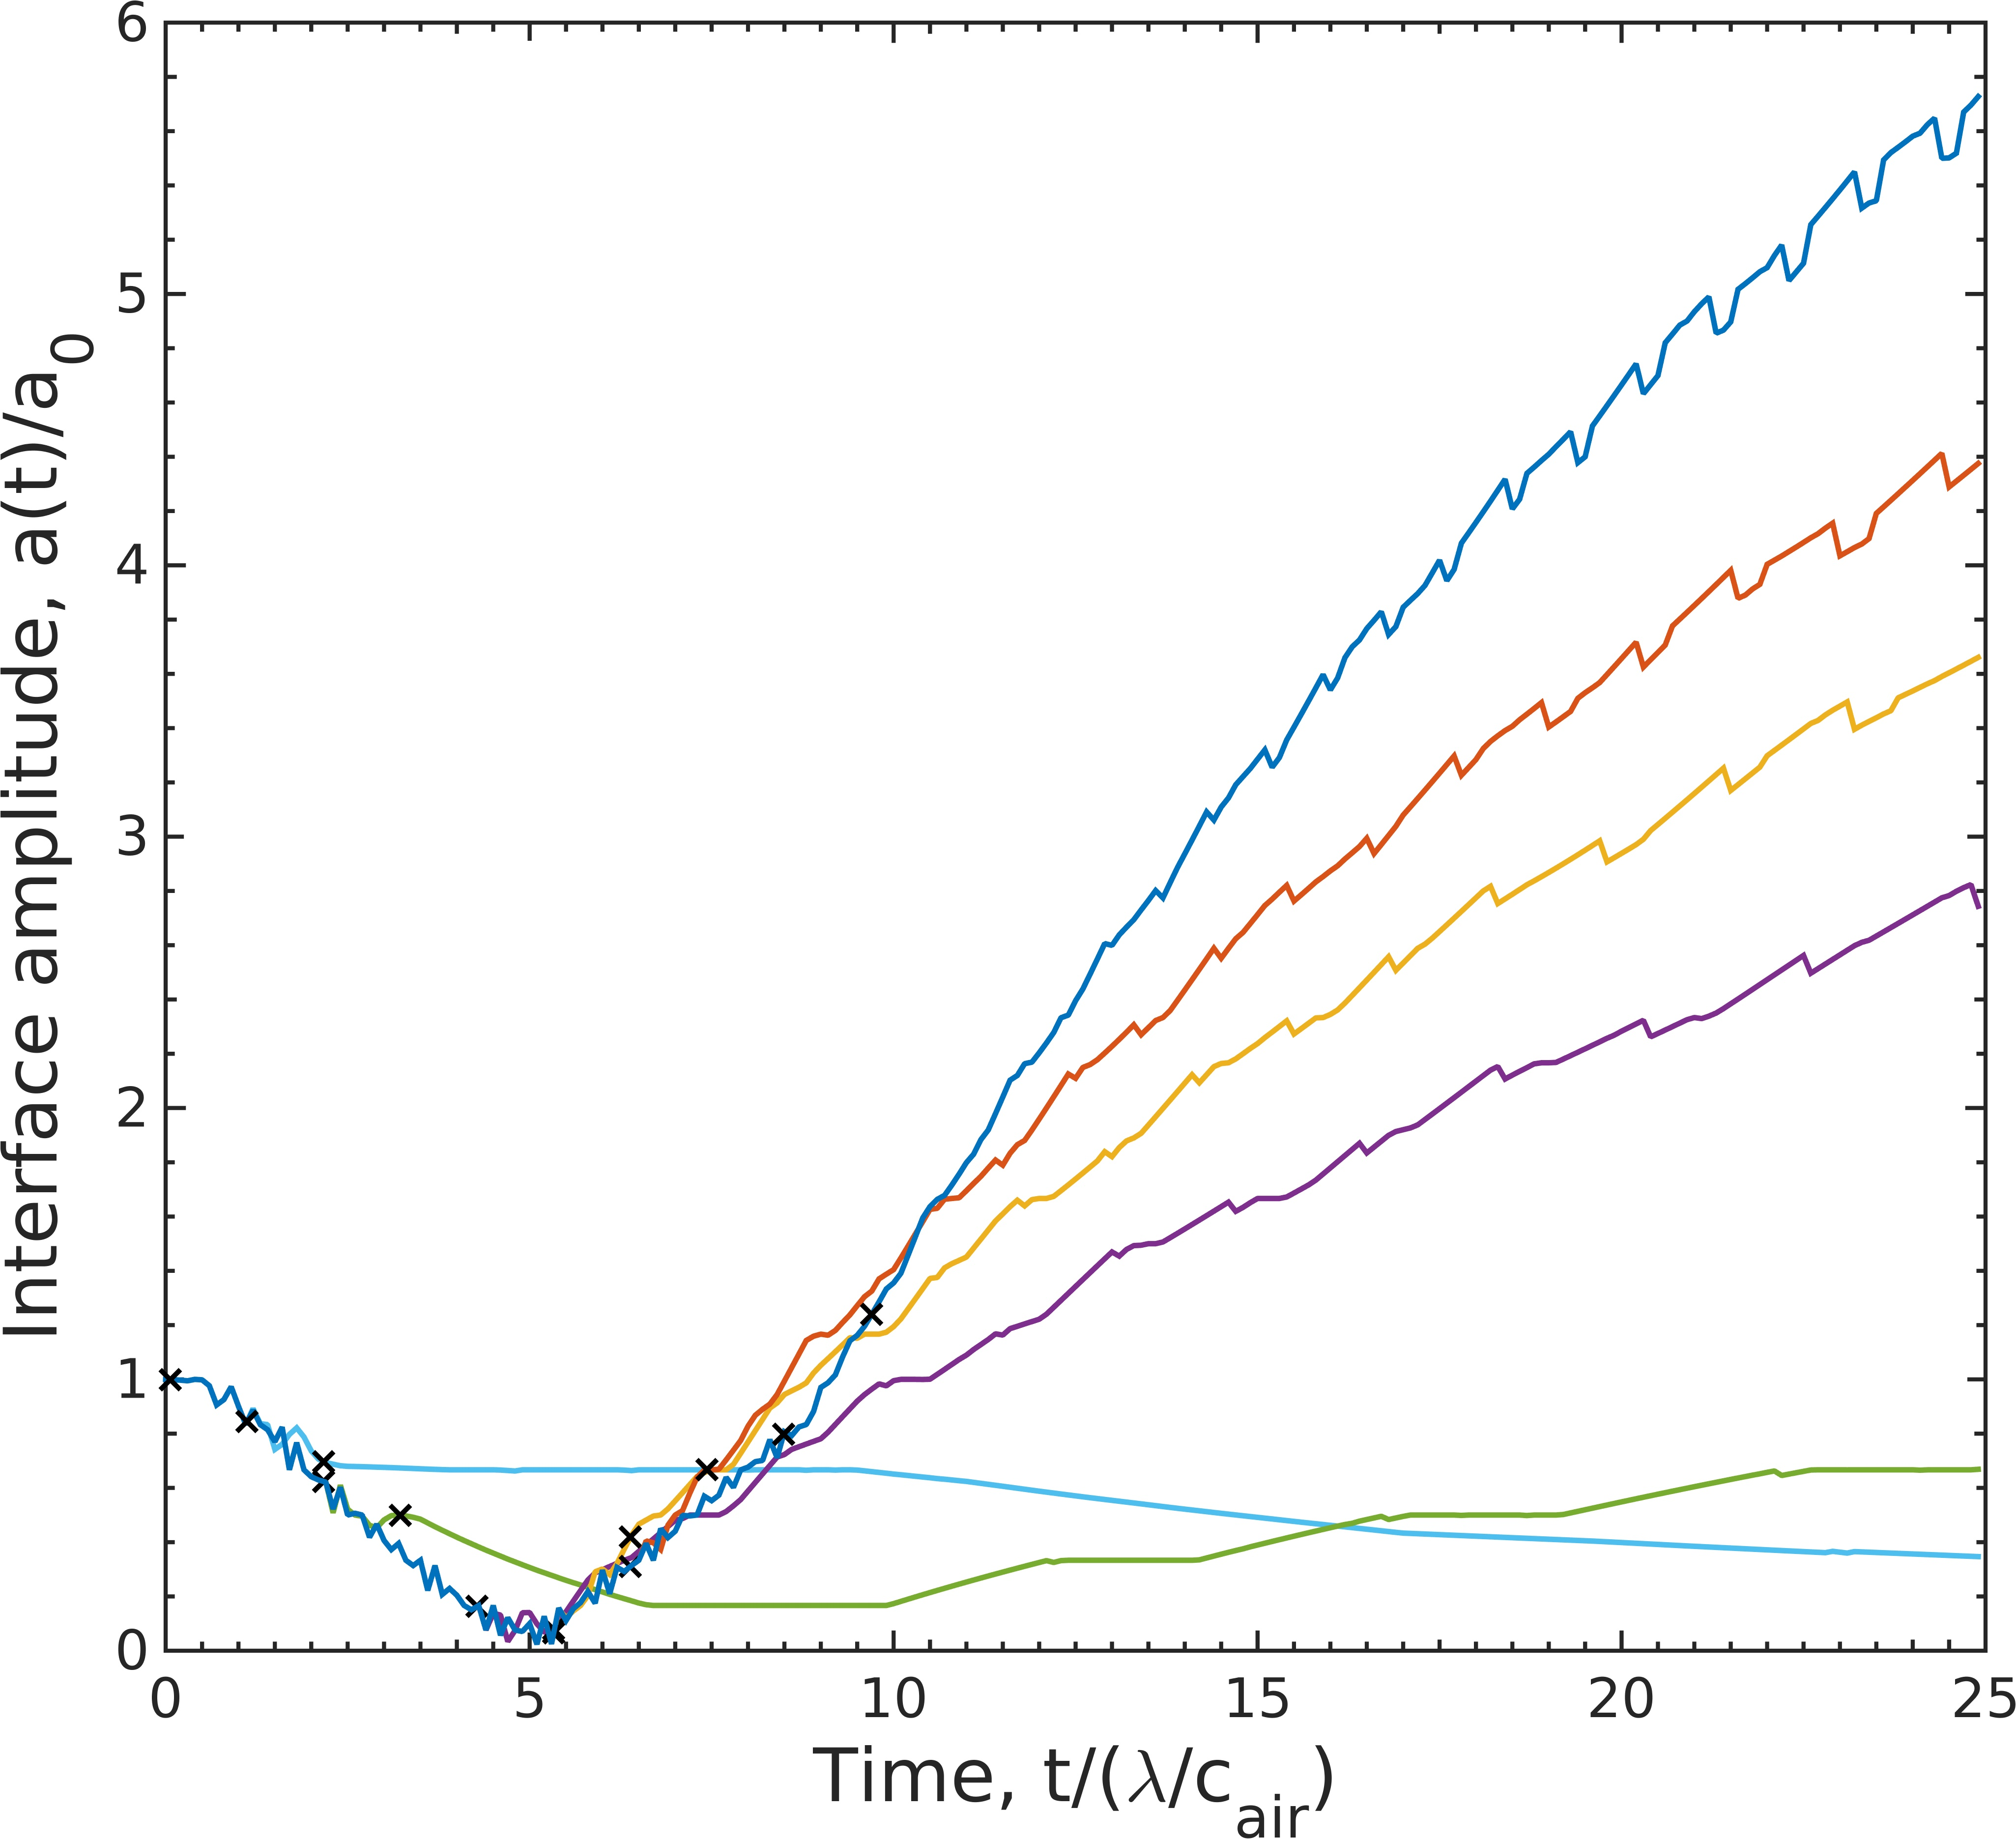
\includegraphics[width=0.48\textwidth]{./figs/lung_figs/interface_multi-lag}
  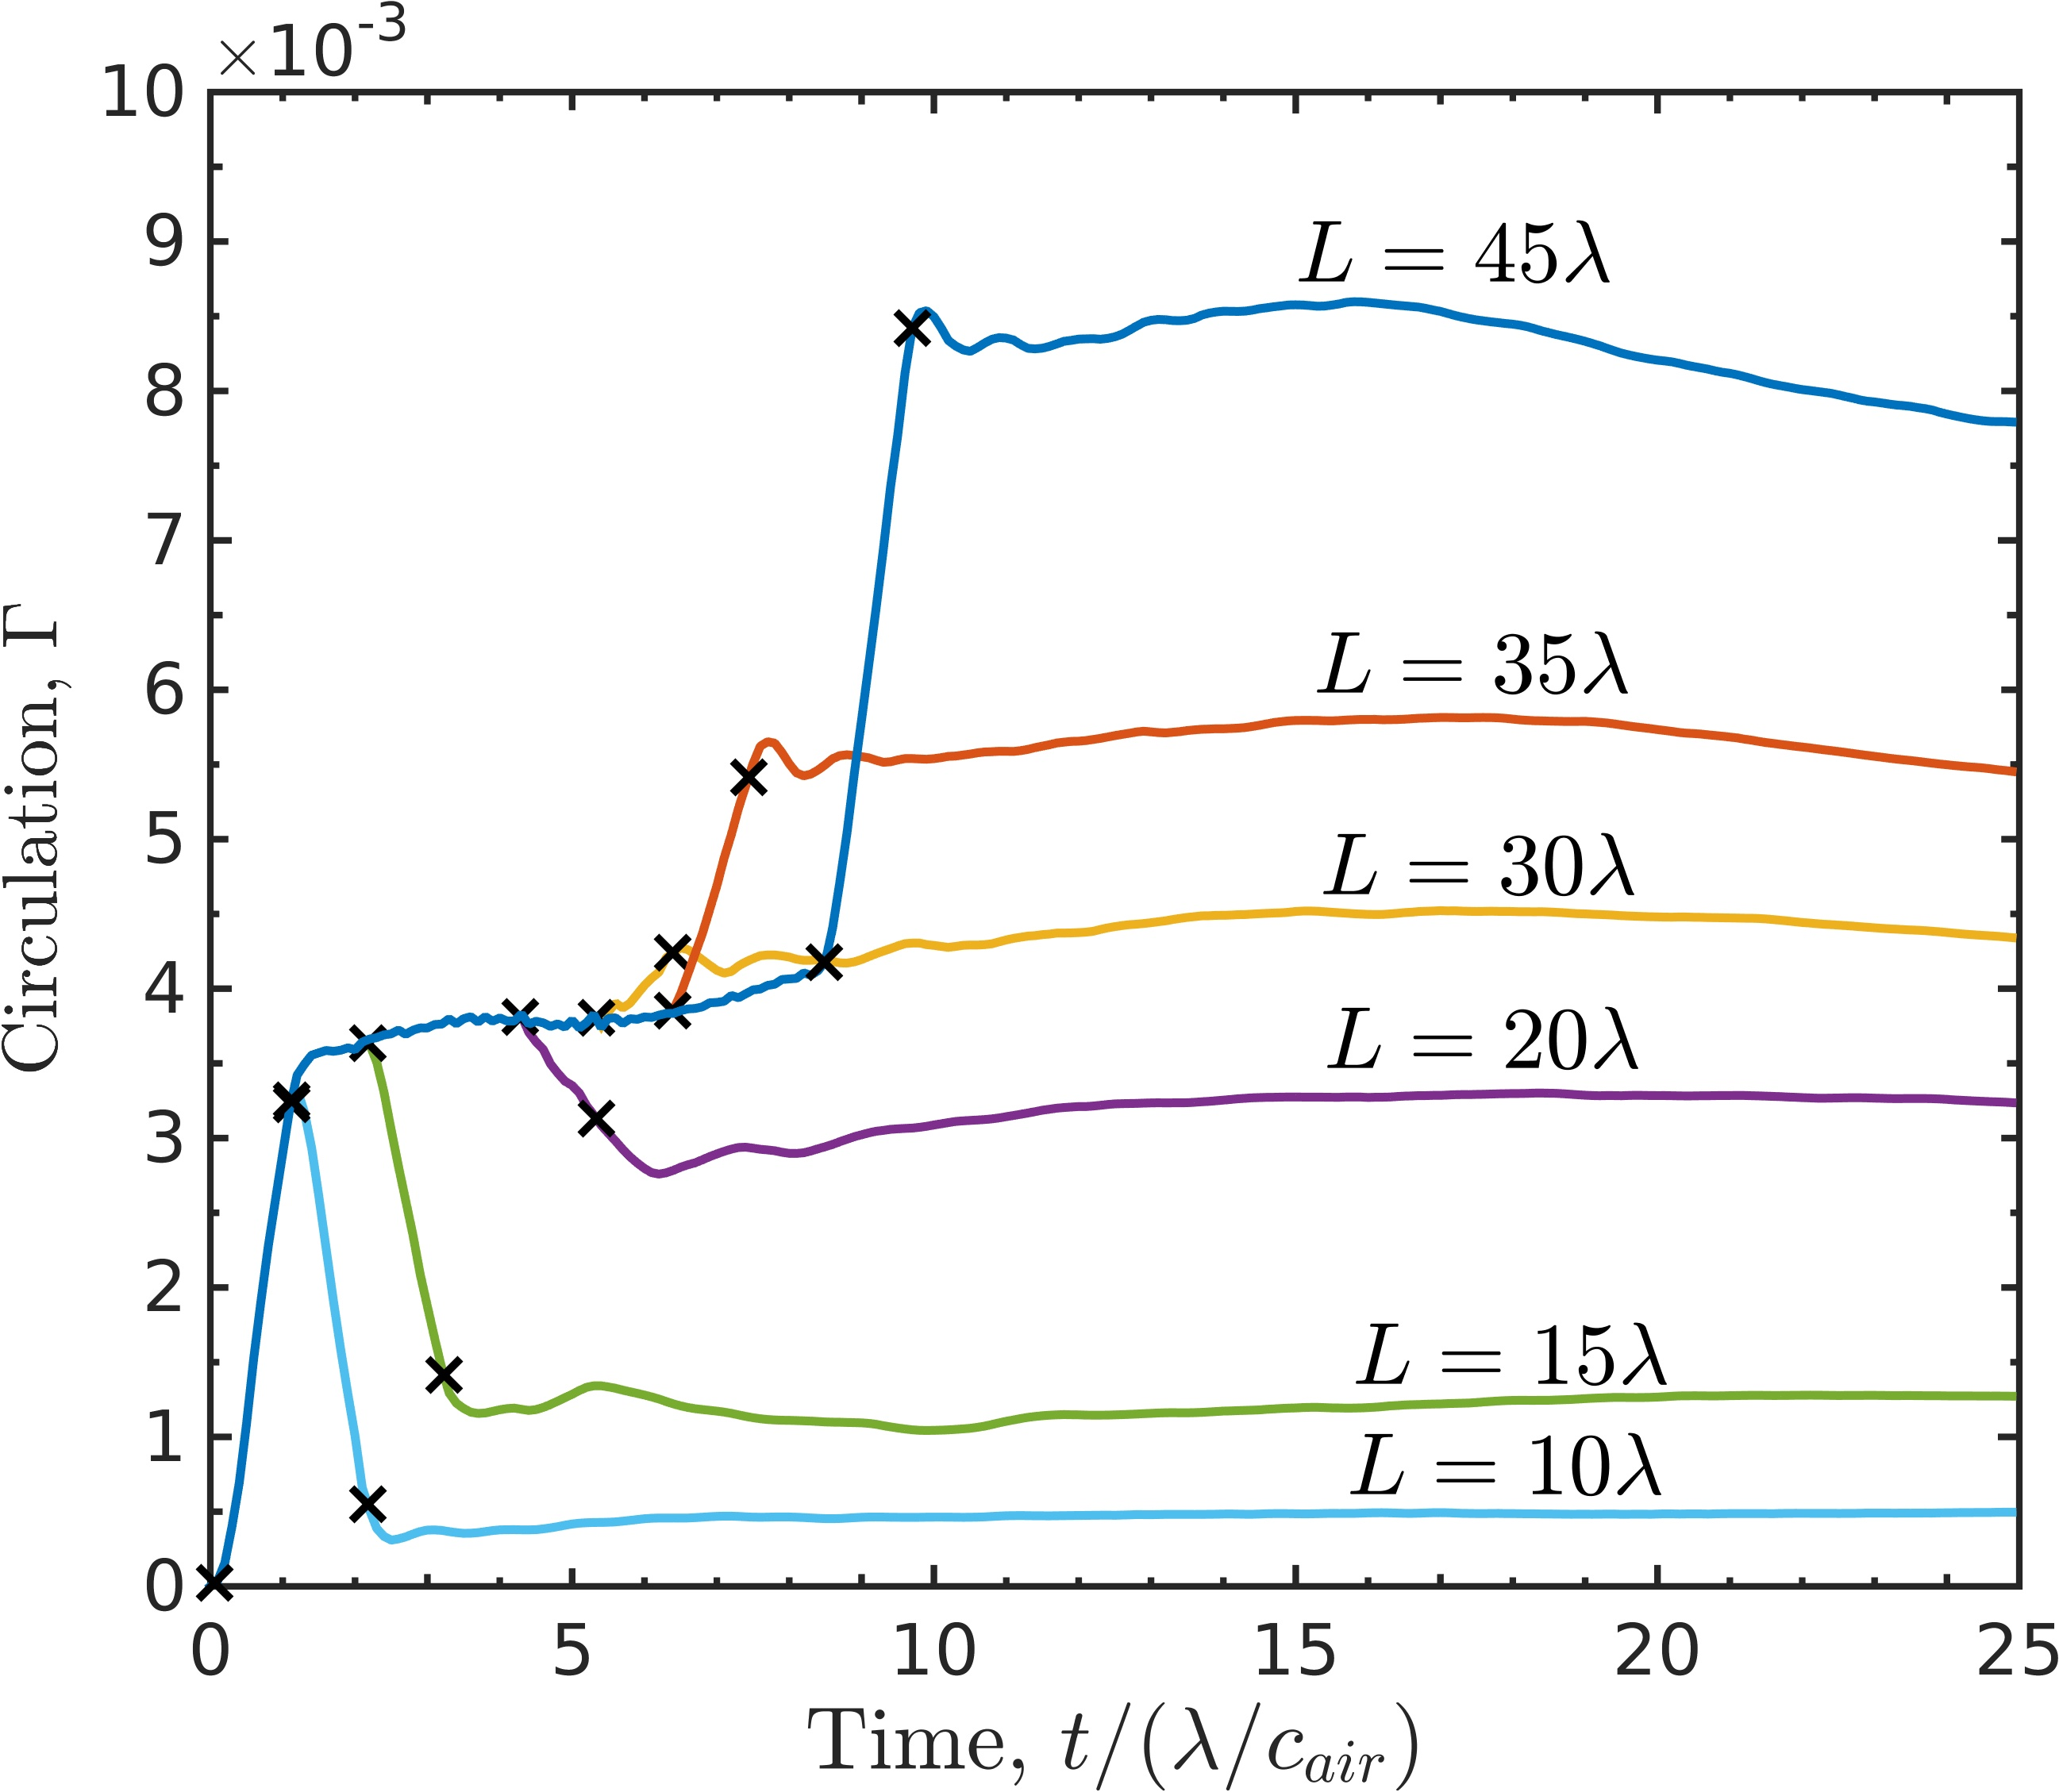
\includegraphics[width=0.48\textwidth]{./figs/lung_figs/circulation_multi-lag_fixed}
  \caption[The interface and circulation dependence on wave
  duration]{The interface amplitude (left) and circulation (right)
    histories for waves of varying total length $L$ and elevated
    static pressure duration between the expansion and compression
    . Here we show results for $L=45\ell$ (blue), $L=35\ell$
    (orange), $L=30\ell$ (yellow), $L=20\ell$ (purple),
    $L=15\ell$ (green), $L=10\ell$ (light blue)}
  \label{fig:trapz_circ_interface_multi-lag}
\end{figure}
Lastly, we investigate the dependence of the interface and circulation
dynamics on the evolution of the interface that occurs during the
wave-interface interaction. To study this, we vary the duration of the
static elevated pressure that the interface experiences between the
compression and expansion of the trapezoidal wave. For our setup, this
is equivalent to changing initial length of the trapezoidal wave $L$,
while keeping constant the wave amplitude $p_a=10$ MPa and the lengths
of the pressure rise and fall $\Delta L_a$. 

Figure \ref{fig:trapz_circ_interface_multi-lag} shows the interface
amplitude and circulation histories corresponding to waves with
$L=45\ell, 35\ell ,30\ell ,25\ell ,15\ell ,10\ell$
for $t\leq 25$.

For the two longest waves, $L=35\ell, 45\ell$, the expansion
encounters the interface appreciably after the perturbation reverses
phase. In these cases, the expansion deposits additional positive
circulation along the right half of the interface. For the shorter
waves, $L \leq 25\ell$, the expansion encounters the interface
before the perturbation reverses phase and the net half-domain
circulation is decreased. For the $L=30\ell$ case, the expansion
hits the interface very shortly after the interface phase-reversal,
when the interface is nearly flat. As a result of this, the pressure
gradient and density gradient are closely aligned and very little
circulation is generated by the expansion wave.

Comparing cases for which the interface inverts phase before
encountering the expansion, the larger $a(t)$ when the expansion
occurs, the more circulation is generated due to the increases
misalignment in density and pressure gradients. The same is true when
comparing cases for which the interface inverts phase before
encountering the expansion.

After the passage of the acoustic wave and all reflections the
pressure returns to the initial, atmospheric conditions. This implies
that the integral of the pressure gradient $\nabla p$ along the
interface, over all time is zero. If the interface remains unchanged
during the interaction with the wave, as it would for a wave moving
with infinite velocity, $\nabla \rho$ would remain constant and the
net baroclinic circulation deposited must be zero. Thus for any finite
duration acoustic wave to deposit net baroclinic circulation upon an
interface, the interface itself must deform during interaction with
the wave. This deformation alters the misalignment of the pressure and
density gradients throughout the passage of the wave such that
vorticity deposited by the compression and expansion waves do not
cancel. This of particular interest for waves in which the pressure
returns to the initial condition after the wave passes, which is not
the case for the traditional shock-accelerated \ac{RMI} problem.

%% Local Variables:
%%% mode: latex
%%% TeX-master: "../main"
%%% End:

